%=====================================================================
%  Resource scaling of the quantum-linear-systems (QSVT) pathway
%  for the viscous Burgers equation
%=====================================================================
\documentclass[11pt,a4paper]{article}

\usepackage[margin=2.4cm]{geometry}
\usepackage{amsmath,amssymb,amsthm,mathtools,bm}
\usepackage{booktabs,array,longtable,multirow}
\usepackage{graphicx}
\usepackage{caption}
\usepackage[dvipsnames]{xcolor}
\usepackage{enumitem}


\usepackage[expansion=false]{microtype}
\usepackage[colorlinks=true,linkcolor=RoyalBlue,citecolor=RoyalBlue,
            urlcolor=RoyalBlue]{hyperref}

% --- float placement: allow text to share pages with tables/figures ---
\renewcommand{\topfraction}{0.9}
\renewcommand{\bottomfraction}{0.8}
\renewcommand{\textfraction}{0.07}
\renewcommand{\floatpagefraction}{0.75}
\setcounter{topnumber}{3}
\setcounter{bottomnumber}{2}
\setcounter{totalnumber}{5}

\theoremstyle{plain}
\newtheorem{proposition}{Proposition}[section]
\newtheorem{lemma}[proposition]{Lemma}
\newtheorem{corollary}[proposition]{Corollary}
\theoremstyle{definition}
\newtheorem{definition}[proposition]{Definition}
\newtheorem{assumption}[proposition]{Assumption}
\theoremstyle{remark}
\newtheorem{remark}[proposition]{Remark}

% ---- macros (every one is also spelled out in the nomenclature table) ----
\newcommand{\R}{\mathbb{R}}
\newcommand{\C}{\mathbb{C}}
\newcommand{\Rey}{\mathrm{Re}}
\newcommand{\Oh}{\mathcal{O}}
\newcommand{\Ot}{\widetilde{\mathcal{O}}}
\newcommand{\ket}[1]{\lvert #1 \rangle}
\newcommand{\bra}[1]{\langle #1 \rvert}
\newcommand{\braket}[2]{\langle #1 \vert #2 \rangle}
\newcommand{\norm}[1]{\lVert #1 \rVert}
\newcommand{\abs}[1]{\lvert #1 \rvert}
\newcommand{\dd}{\mathrm{d}}
\newcommand{\ii}{\mathrm{i}}
\newcommand{\Id}{\mathbb{I}}
\newcommand{\uvec}{\bm{u}}
\newcommand{\yvec}{\bm{y}}
\newcommand{\Lmat}{\mathsf{L}}
\newcommand{\Amat}{\mathsf{A}}
\newcommand{\Fone}{\mathsf{F}_1}
\newcommand{\Ftwo}{\mathsf{F}_2}
\newcommand{\kQ}{\kappa_{\textsc{q}}}

\title{\bf Resource scaling of the quantum-linear-systems pathway\\
for the viscous Burgers equation\\[2mm]
\large An error budget and complexity analysis of the
block-encoding\,+\,QSVT method,\\ with comparison to classical solvers
and to Koopman--von~Neumann linearisation}

\author{Prepared as a technical report for the\\
Niels Bohr Quantum Summer School challenge\\
\emph{Quantum simulation of non-linear PDEs}}

\date{\today}

\begin{document}
\maketitle

\begin{abstract}
\noindent
Setty [\emph{J.~Phys.~A: Math.\ Theor.}\ \textbf{59}, 185303 (2026)] proposes a
pathway that solves differential equations on a quantum computer by
discretising them into a linear system $\Lmat\yvec=\bm{b}$, block-encoding
$\Lmat$, and inverting it with the quantum singular value transformation
(QSVT); nonlinear equations are brought into this form by Carleman
linearisation.  That work demonstrates the pathway at circuit level on a
$30\times30$ instance of the viscous Burgers equation and reports two-qubit
gate depths, but it does not derive how the cost scales.  This report supplies
that analysis.  We enumerate every error source in the pipeline, show which of
them are amplified by the condition number, and derive the qubit count, the
block-encoding subnormalisation, the polynomial degree, the circuit depth, the
post-selection success probability and the sample complexity as explicit
functions of the target error $\epsilon$, the Reynolds number $\Rey$, the grid
size and the Carleman order.  Every formula is validated numerically against the
published instance; our success-probability model reproduces the reported value
to $5\%$ and our subnormalisation formula is exact.  Four findings stand out.
(i) The quantity that sets the QSVT polynomial degree is
$\alpha/\sigma_{\min}$, not $\sigma_{\max}/\sigma_{\min}$; the two differ by a
factor of $3.5$ in the published instance.  (ii) With the coherent-permutation
block encoding used in the paper, the subnormalisation grows as
$n_x^{N-1}$ with grid size $n_x$ and Carleman order $N$, which erases the
nominal exponential compression; replacing it with an arithmetic sparse-access
oracle restores an $\Oh(N^2)$ scaling.  (iii) Solving one time step at a time,
as the paper does, makes the success probability decay as $p_s^{m}$ over $m$
steps and is not viable; a dilated ``history-state'' system is required, and we
show that the product of subnormalisation and step count entering its condition
number is independent of the time step.  (iv) The Carleman convergence
criterion evaluates to $\Rey<\pi/2$ for this discretisation, so the published
instance ($\Rey=100$) lies far outside the regime in which the linearisation is
provably convergent.  Assembling everything, the sequential gate depth scales as
$\Ot\!\left(\kappa_V\,T\,\Rey^{-1}\epsilon^{-1}N^5\right)$ against a classical
pseudo-spectral cost of $\Ot(T\epsilon^{-1})$ arithmetic operations: in one
space dimension there is no speedup of any kind.  We close by explaining what
changes for Koopman--von~Neumann linearisation --- the derivation transfers
almost verbatim, but the state space grows as $M^{n_x}$ rather than $n_x^N$ ---
and by listing the specific changes that would be needed for the pathway to
become competitive.
\end{abstract}

\tableofcontents

%=====================================================================
\section{Introduction and scope}
%=====================================================================

\subsection{What problem this report addresses}

Quantum computers evolve states linearly.  A nonlinear partial differential
equation (PDE) therefore cannot be simulated directly; it must first be
\emph{embedded} in a linear problem, and only then handed to a quantum
subroutine.  The pathway analysed here, due to Setty~\cite{Setty2026}, chains
together four such steps for the one-dimensional viscous Burgers equation:

\begin{center}
\framebox{\parbox{0.93\textwidth}{\centering
PDE $\;\xrightarrow{\text{finite differences}}\;$ quadratic ODE system
$\;\xrightarrow{\text{Carleman}}\;$ linear ODE system
$\;\xrightarrow{\text{implicit time stepping}}\;$ linear algebraic system
$\;\xrightarrow{\text{block encoding + QSVT}}\;$ quantum state}}
\end{center}

Reference~\cite{Setty2026} establishes that this chain \emph{works}: it
constructs the explicit gate-level circuit for a $30\times30$ Burgers instance,
runs it in simulation, and reports the resulting two-qubit gate depths on two
IBM processor topologies.  What it does not do --- and what the present report
supplies --- is derive how each resource behaves as the instance is made larger
and more accurate.  Without that, one cannot say whether the pathway is a
promising route to quantum advantage or a demonstration that happens to fit on
eleven qubits.

The analysis is written at the level of a master's student in physics.  Every
symbol is defined before it is used, and every piece of background that goes
beyond a first course in numerical methods and quantum computing is developed in
an appendix rather than cited.  Section~\ref{sec:nomenclature} collects all
notation in one table for reference.

\subsection{What is assumed known, and what is developed here}

We assume the reader is comfortable with linear algebra (eigenvalues, singular
values, matrix norms), with the idea of a finite-difference approximation to a
derivative, and with the basic formalism of quantum computing (qubits, unitary
gates, measurement, the Dirac notation $\ket{\psi}$).  Everything else is built
up:

\begin{itemize}[nosep,leftmargin=*]
\item Appendix~\ref{app:fd} --- finite-difference stencils and their truncation
      errors, including the Gronwall argument that converts a local error into a
      global one.
\item Appendix~\ref{app:kron} --- the Kronecker product algebra needed to
      manipulate the Carleman blocks.
\item Appendix~\ref{app:spectra} --- exact spectra of the discrete diffusion and
      Carleman operators.
\item Appendix~\ref{app:qsvt} --- quantum signal processing, QSVT, and the
      polynomial approximation of $1/x$.
\item Appendix~\ref{app:be} --- what a block encoding is, and the two concrete
      constructions we compare.
\item Appendix~\ref{app:aa} --- amplitude amplification and amplitude
      estimation, and why they enter the sample complexity.
\item Appendix~\ref{app:pert} --- the perturbation bound that explains why some
      errors get multiplied by the condition number and others do not.
\item Appendix~\ref{app:colehopf} --- the Cole--Hopf transformation, which is
      the reason Burgers is an unrepresentative test case.
\item Appendix~\ref{app:numerics} --- the numerical scripts used to validate
      every formula in the report.
\end{itemize}

\subsection{Summary of findings}
\label{sec:summary}

For the reader who wants the conclusions before the derivations:

\begin{enumerate}[leftmargin=*]

\item \textbf{The relevant condition number is $\alpha/\sigma_{\min}$.}
The QSVT polynomial degree is set not by the classical condition number
$\sigma_{\max}/\sigma_{\min}$ of the linear system, but by the ratio of the
block-encoding subnormalisation $\alpha$ to the smallest singular value.  For
the published Burgers instance these are $5.46$ and $1.57$ respectively --- a
factor $3.5$ apart.  The former matches the design value $\kappa=8$ used in
\cite{Setty2026}; the latter does not (Section~\ref{sec:kappa}).

\item \textbf{The block encoding, not the matrix, is the bottleneck.}
For the coherent-permutation block encoding of \cite{Setty2026,Setty2025BE} we
derive and numerically confirm
$\alpha \simeq n_x^{\,N-1}\lambda_{\rm cfl}$,
where $n_x$ is the number of interior grid points, $N$ the Carleman order and
$\lambda_{\rm cfl}=\Delta t/\Delta x$ the Courant number.  Because $\alpha$
enters the cost linearly, the algorithm is \emph{polynomial in the grid size and
exponential in the Carleman order} --- exactly the scaling the Carleman
embedding was supposed to avoid.  An arithmetic sparse-access oracle instead
gives $\alpha=\Oh(N^2\lambda_{\rm diff})$, independent of $n_x$ except through
the diffusion number (Section~\ref{sec:two-be}).

\item \textbf{Sequential time stepping does not scale.}
Reference~\cite{Setty2026} solves one implicit step at a time.  Because each
solve is heralded with probability $p_s<1$ and the output of one step is the
input of the next, chaining $m$ steps costs $\Oh(p_s^{-m/2})$ even with optimal
amplitude amplification.  The dilated ``history-state'' formulation removes
this, and we show that the product $\alpha m$ entering its condition number is
\emph{independent of $\Delta t$}, which is what makes the whole pathway
tractable at all (Section~\ref{sec:sequential}).

\item \textbf{Carleman convergence requires $\Rey<\pi/2$.}
Evaluating the standard convergence ratio for this specific discretisation gives
$R_\star = 2\Rey/\pi$, so the Carleman series has a provable convergence regime
only for $\Rey\lesssim1.6$.  The instance in \cite{Setty2026} has $\Rey=100$,
giving $R_\star\approx64$; we confirm numerically that the ratio computed
directly from the matrices is $76$.  The published example is a circuit
demonstration, not a converged simulation, and should not be read otherwise
(Section~\ref{sec:carleman-err}).

\item \textbf{No speedup in one dimension.}
Assembling all of the above, the quantum sequential depth is
$\Ot(\kappa_V T\Rey^{-1}\epsilon^{-1}N^5)$ logical two-qubit gates, against
$\Ot(T\epsilon^{-1})$ floating-point operations for a classical pseudo-spectral
solver.  The $\epsilon$ scaling is identical, the quantum route carries extra
factors of $N^5$ and of the eigenvector condition number $\kappa_V$, and it
returns a quantum state rather than the field.  A crossover can only be sought
in $d\ge3$ spatial dimensions with observable-only readout
(Section~\ref{sec:classical}).

\end{enumerate}

\begin{remark}[On tone]
None of this is a criticism of \cite{Setty2026}, whose stated purpose is to
consolidate the pathway and provide gate-level resource estimates for small
instances --- a genuinely useful contribution, and one whose published numbers
we rely on throughout as calibration data.  The scaling questions were simply
left open, and answering them honestly is the point of this report.
\end{remark}

%=====================================================================
\section{Problem statement and notation}
%=====================================================================

\subsection{The equation and the deliverable}

We study the one-dimensional viscous Burgers equation
\begin{equation}
\frac{\partial u}{\partial t} + u\,\frac{\partial u}{\partial x}
= \nu\,\frac{\partial^2 u}{\partial x^2},
\qquad x\in[0,L],\quad t\in[0,T],
\label{eq:burgers}
\end{equation}
where
\begin{itemize}[nosep,leftmargin=*]
\item $u=u(t,x)\in\R$ is the unknown scalar field (a velocity);
\item $\nu>0$ is the kinematic viscosity (units: length$^2$/time);
\item $L>0$ is the length of the spatial domain;
\item $T>0$ is the final time at which we want the solution.
\end{itemize}
The initial condition is $u(0,x)=u_0(x)$, taken smooth, with amplitude
\begin{equation}
U := \norm{u_0}_\infty = \max_{x\in[0,L]}\abs{u_0(x)} .
\end{equation}
Reference~\cite{Setty2026} imposes homogeneous Dirichlet conditions
$u(t,0)=u(t,L)=0$; the challenge specification uses periodic conditions
$u(t,0)=u(t,L)$.  The two differ only in the boundary rows of the matrices below
and change none of the scaling results, so we carry the Dirichlet case (to match
the paper we are analysing) and flag the two places where periodicity would
alter a constant.

The nonlinear term $u\,\partial_x u$ is what makes this hard: it is quadratic in
$u$, and a quantum computer applies linear maps.  The diffusive term
$\nu\,\partial_{xx}u$ is linear and, crucially, \emph{dissipative} --- it damps
the solution --- which is what makes the Carleman embedding of
Section~\ref{sec:carleman} converge at all.

\paragraph{Deliverable.}  Following the challenge specification, we are given an
oracle that prepares the amplitude encoding of the initial data,
\begin{equation}
\mathcal{U}_{0}:\ \ket{0}\ \longmapsto\
\frac{1}{\norm{\uvec_0}_2}\sum_{j=0}^{n_x-1} u_0(x_j)\,\ket{j},
\label{eq:oracle}
\end{equation}
where $x_j$ are the grid points defined in Section~\ref{sec:space} and
$\uvec_0\in\R^{n_x}$ is the vector of initial values, and we must produce the
amplitude encoding of a numerical approximation to $u(T,\cdot)$,
\begin{equation}
\ket{\hat u(T)}\ =\ \frac{1}{\norm{\hat\uvec(T)}_2}
\sum_{j=0}^{n_x-1}\hat u_j(T)\,\ket{j},
\label{eq:target}
\end{equation}
together with honest estimates of the resources required.  We write $\hat{\cdot}$
throughout for a numerically computed approximation, reserving unhatted symbols
for exact quantities.

\paragraph{Accuracy target.}  We measure error in the relative discrete
$\ell^2$ norm,
\begin{equation}
\epsilon \;:=\;
\frac{\norm{\hat\uvec(T)-\uvec^{\rm exact}(T)}_2}{\norm{\uvec^{\rm exact}(T)}_2},
\qquad
\norm{\bm{v}}_2 := \Big(\textstyle\sum_j \abs{v_j}^2\Big)^{1/2},
\label{eq:epsdef}
\end{equation}
where $\uvec^{\rm exact}(T)$ denotes the exact PDE solution sampled on the grid.
This is the natural norm here because it is the one the amplitude encoding
\eqref{eq:target} actually represents.

\subsection{Non-dimensionalisation}

It is much easier to read the scaling results if the problem carries only one
physical parameter.  Introduce dimensionless variables
\begin{equation}
\bar x = \frac{x}{L},\qquad
\bar t = \frac{tU}{L},\qquad
\bar u = \frac{u}{U},
\end{equation}
so that $\bar x\in[0,1]$.  Substituting into \eqref{eq:burgers} and using the
chain rule ($\partial_t = (U/L)\partial_{\bar t}$,
$\partial_x = (1/L)\partial_{\bar x}$) gives
\begin{equation}
\frac{U^2}{L}\frac{\partial\bar u}{\partial\bar t}
+ \frac{U^2}{L}\,\bar u\frac{\partial\bar u}{\partial\bar x}
= \frac{\nu U}{L^2}\frac{\partial^2\bar u}{\partial\bar x^2}
\quad\Longleftrightarrow\quad
\frac{\partial\bar u}{\partial\bar t}
+ \bar u\frac{\partial\bar u}{\partial\bar x}
= \frac{1}{\Rey}\frac{\partial^2\bar u}{\partial\bar x^2},
\end{equation}
where the single remaining parameter is the \textbf{Reynolds number}
\begin{equation}
\boxed{\ \Rey := \frac{UL}{\nu}\ }
\label{eq:Re}
\end{equation}
which measures the strength of the nonlinear (advective) term relative to the
linear (diffusive) one.  From here on we drop the bars and work in
dimensionless variables, i.e.\ $U=L=1$ and $\nu=1/\Rey$.  Reference
\cite{Setty2026} uses $L=1$, $U=1$, $\nu=0.01$, hence $\Rey=100$.

\begin{remark}[Why $\Rey$ is the parameter that matters]
Everything difficult about \eqref{eq:burgers} is controlled by $\Rey$.  At small
$\Rey$ diffusion dominates, the solution stays smooth and decays, and (as we
show in Section~\ref{sec:carleman-err}) the Carleman embedding converges.  At
large $\Rey$ the nonlinearity steepens the profile into a thin internal layer of
width $\sim\Rey^{-1}$, which must be resolved by the grid \emph{and} which drives
the Carleman series out of its radius of convergence.  Nearly every cost in this
report is really a cost in $\Rey$.
\end{remark}

\subsection{Nomenclature}
\label{sec:nomenclature}

Table~\ref{tab:nomen} lists every symbol used in this report, in order of first
appearance.  Readers may prefer to skip it now and consult it as needed.

\begin{table}[htbp]
\centering
\caption{Nomenclature.  ``§'' gives the section where the symbol is defined.}
\label{tab:nomen}
\small
\begin{tabular}{@{}llc@{}}
\toprule
Symbol & Meaning & § \\
\midrule
\multicolumn{3}{@{}l}{\emph{Continuum problem}}\\
$u(t,x)$ & scalar field solving Burgers' equation & 2.1\\
$\nu$ & kinematic viscosity & 2.1\\
$L,\ T$ & domain length, final time & 2.1\\
$U$ & amplitude $\norm{u_0}_\infty$ of the initial data & 2.1\\
$\Rey$ & Reynolds number $UL/\nu$ & 2.2\\
$\epsilon$ & target relative $\ell^2$ error at time $T$ & 2.1\\
$\delta_{\rm v}$ & viscous-layer thickness, $\delta_{\rm v}\sim L/\Rey$ & 4.2\\
\midrule
\multicolumn{3}{@{}l}{\emph{Discretisation}}\\
$n_x$ & number of interior spatial grid points & 3.1\\
$\Delta x$ & grid spacing $L/(n_x+1)$ & 3.1\\
$q$ & spatial qubits, $q=\lceil\log_2 n_x\rceil$ & 3.1\\
$\uvec(t)$ & vector $(u_1,\dots,u_{n_x})^{\!\top}$ of nodal values & 3.1\\
$\Fone,\Ftwo$ & linear and quadratic coefficient matrices & 3.1\\
$\lambda_1,\lambda_2$ & $\nu/\Delta x^2$ and $-1/(2\Delta x)$ & 3.1\\
$\Delta t$ & time step & 3.3\\
$m$ & number of time steps, $m=T/\Delta t$ & 3.3\\
$\lambda_{\rm diff}$ & diffusion number $\nu\Delta t/\Delta x^2$ & 3.3\\
$\lambda_{\rm cfl}$ & Courant number $\Delta t/\Delta x$ & 3.3\\
\midrule
\multicolumn{3}{@{}l}{\emph{Carleman embedding}}\\
$N$ & Carleman truncation order & 3.2\\
$\hat y_j$ & $j$-th Carleman block, $\uvec^{\otimes j}$ & 3.2\\
$\yvec$ & stacked Carleman vector $(\hat y_1;\dots;\hat y_N)$ & 3.2\\
$\Amat$ & Carleman matrix & 3.2\\
$A^j_k$ & block of $\Amat$ mapping $\hat y_k\to\dot{\hat y}_j$ & 3.2\\
$D$ & dimension of $\Amat$, $D=\Oh(n_x^N)$ & 3.2\\
$R,\ R_\star$ & Carleman convergence ratios & 4.3\\
$\gamma$ & $\norm{\uvec}_2$, controls block-1 readout & 5.6\\
$P_1$ & probability of the first Carleman block & 5.6\\
\midrule
\multicolumn{3}{@{}l}{\emph{Linear system and quantum algorithm}}\\
$\Lmat$ & implicit-step matrix $\Id-\Delta t\,\Amat$ & 3.3\\
$\mathcal{L}$ & dilated (history-state) matrix & 5.7\\
$\alpha$ & block-encoding subnormalisation & 3.4\\
$s$ & maximum number of nonzeros per row of $\Lmat$ & 3.4\\
$n_{\rm data}$ & number of distinct (value, offset) pairs & 5.3\\
$m_{\rm flag}$ & flag qubits (data $+$ delete) & 5.1\\
$q_M$ & matrix-register qubits, $q_M=\lceil\log_2 D\rceil$ & 5.1\\
$\sigma_k$ & singular values of $\Lmat^\dagger\!/\alpha$ & 3.5\\
$\kQ$ & effective condition number $\alpha/\sigma_{\min}(\Lmat)$ & 5.2\\
$\kappa_V$ & eigenvector condition number of $\Amat$ & 5.7\\
$d$ & degree of the QSVT inverse polynomial & 3.5\\
$\beta$ & QSP normalisation of the $1/x$ polynomial & 3.5\\
$p_s$ & QSVT post-selection success probability & 3.5\\
$p_{\rm tot}$ & total success probability & 5.6\\
$D_{\rm BE},D_\Pi,D_{\rm QSVT}$ & two-qubit depths & 5.5\\
$M_{\rm shot}$ & number of measurement repetitions & 5.8\\
\bottomrule
\end{tabular}
\end{table}

%=====================================================================
\section{The pathway, stage by stage}
\label{sec:pathway}
%=====================================================================

This section restates the method of \cite{Setty2026} with every step made
explicit, because the resource analysis in Sections~\ref{sec:errors} and
\ref{sec:resources} refers to the individual stages.  A reader already familiar
with the paper can skim to Section~\ref{sec:reference}, where we reproduce its
published instance numerically.

\subsection{Stage 1: spatial discretisation}
\label{sec:space}

Place $n_x$ interior grid points on $[0,L]$,
\begin{equation}
x_j = j\,\Delta x,\quad j=1,\dots,n_x,
\qquad \Delta x := \frac{L}{n_x+1},
\end{equation}
with $x_0=0$ and $x_{n_x+1}=L$ carrying the boundary values.  Write
$u_j(t)\approx u(t,x_j)$ and collect them in
$\uvec(t)=(u_1,\dots,u_{n_x})^{\!\top}\in\R^{n_x}$.  Replace the derivatives by
second-order central differences (derived in Appendix~\ref{app:fd}),
\begin{equation}
\frac{\partial u}{\partial x}\Big|_{x_j}\!\approx\frac{u_{j+1}-u_{j-1}}{2\Delta x},
\qquad
\frac{\partial^2u}{\partial x^2}\Big|_{x_j}\!\approx
\frac{u_{j+1}-2u_j+u_{j-1}}{\Delta x^2},
\label{eq:stencils}
\end{equation}
each accurate to $\Oh(\Delta x^2)$.  Substituting into \eqref{eq:burgers} gives
the semi-discrete system used in \cite[Eq.~(F.2)]{Setty2026},
\begin{equation}
\frac{\dd u_j}{\dd t}
= \underbrace{\frac{\nu}{\Delta x^{2}}\bigl(u_{j+1}-2u_j+u_{j-1}\bigr)}_{\text{diffusion}}
\;-\;\underbrace{\frac{1}{2\Delta x}\,u_j\bigl(u_{j+1}-u_{j-1}\bigr)}_{\text{advection}},
\qquad j=1,\dots,n_x .
\label{eq:semidiscrete}
\end{equation}
This is a system of $n_x$ coupled ordinary differential equations (ODEs) whose
right-hand side is a \emph{quadratic polynomial} in the unknowns.  Writing it in
the standard quadratic form
\begin{equation}
\boxed{\ \frac{\dd\uvec}{\dd t} = \Fone\,\uvec + \Ftwo\,\uvec^{\otimes2}\ }
\label{eq:quadode}
\end{equation}
(the notation $\uvec^{\otimes2}:=\uvec\otimes\uvec\in\R^{n_x^2}$, the vector of
all pairwise products $u_iu_j$, is explained in Appendix~\ref{app:kron}) we
read off, with
\begin{equation}
\lambda_1 := \frac{\nu}{\Delta x^{2}},
\qquad
\lambda_2 := -\frac{1}{2\Delta x},
\end{equation}
the coefficient matrices \cite[Eqs.~(F.3)--(F.4)]{Setty2026}
\begin{equation}
\Fone=\lambda_1\!
\begin{pmatrix}
-2 & 1 & & \\
1 & -2 & 1 & \\
& \ddots&\ddots&\ddots\\
& & 1 & -2
\end{pmatrix}\in\R^{n_x\times n_x},
\qquad
[\Ftwo]_{i,\,i\,n_x+j}=
\begin{cases}
+\lambda_2, & j=i+1,\\
-\lambda_2, & j=i-1,\\
0,&\text{otherwise,}
\end{cases}
\label{eq:F1F2}
\end{equation}
with $\Ftwo\in\R^{n_x\times n_x^2}$.  The index pattern of $\Ftwo$ says exactly
what \eqref{eq:semidiscrete} says: the $i$-th output picks out the products
$u_iu_{i+1}$ and $u_iu_{i-1}$.

\begin{remark}[Conservative versus advective form]
\label{rem:conservative}
Equation~\eqref{eq:semidiscrete} discretises $u\,\partial_xu$ directly
(``advective form'').  The algebraically equivalent ``conservative form''
$\tfrac12\partial_x(u^2)$ discretises to
$-\frac{1}{4\Delta x}(u_{j+1}^2-u_{j-1}^2)$ and has the advantage of exactly
preserving a discrete analogue of the energy bound $\norm{u(t)}_2\le\norm{u_0}_2$.
Since the challenge specification supplies exactly that bound as the property
that makes efficient simulation possible, the conservative (or the skew-symmetric
average of the two) form is the better choice in practice.  It changes the
entries of $\Ftwo$ but not its sparsity pattern, so all scaling results below are
unaffected; we keep the advective form to match \cite{Setty2026}.
\end{remark}

\subsection{Stage 2: Carleman linearisation}
\label{sec:carleman}

\paragraph{The idea.}  Equation~\eqref{eq:quadode} is nonlinear only because of
the term $\Ftwo\uvec^{\otimes2}$.  Carleman's observation is that if we
\emph{treat the products as new unknowns}, the equations governing them are
again polynomial, and the whole system becomes linear --- at the price of
infinitely many variables.  Define the Carleman blocks
\begin{equation}
\hat y_j(t) := \uvec(t)^{\otimes j}\in\R^{n_x^j},\qquad j=1,2,3,\dots
\end{equation}
so $\hat y_1=\uvec$, $\hat y_2$ holds all quadratic monomials $u_au_b$,
$\hat y_3$ all cubic monomials, and so on.

\paragraph{The hierarchy.}  Differentiating $\hat y_j$ with the product rule
(Appendix~\ref{app:kron}, Lemma~\ref{lem:prodrule}) gives
\begin{equation}
\frac{\dd\hat y_j}{\dd t}
=\sum_{v=0}^{j-1}
\uvec^{\otimes v}\otimes\dot{\uvec}\otimes\uvec^{\otimes(j-1-v)} ,
\end{equation}
and substituting $\dot{\uvec}=\Fone\uvec+\Ftwo\uvec^{\otimes2}$ into each slot,
\begin{equation}
\boxed{\ \frac{\dd\hat y_j}{\dd t}= A^j_j\,\hat y_j + A^j_{j+1}\,\hat y_{j+1}\ }
\label{eq:hierarchy}
\end{equation}
with the blocks \cite[Eqs.~(E.4)--(E.5)]{Setty2026}
\begin{align}
A^j_j &= \sum_{v=0}^{j-1}
\Id^{\otimes v}\otimes\Fone\otimes\Id^{\otimes(j-1-v)}
\ \in\R^{n_x^j\times n_x^j},
\label{eq:Ajj}\\
A^j_{j+1} &= \sum_{v=0}^{j-1}
\Id^{\otimes v}\otimes\Ftwo\otimes\Id^{\otimes(j-1-v)}
\ \in\R^{n_x^j\times n_x^{j+1}},
\label{eq:Ajj1}
\end{align}
where $\Id$ is the $n_x\times n_x$ identity.

The structure of \eqref{eq:hierarchy} is worth pausing on, because it is the
single most important fact about the method.  Substituting the \emph{linear}
part $\Fone\uvec$ into a degree-$j$ product leaves the degree at $j$: that term
closes on $\hat y_j$ itself.  Substituting the \emph{quadratic} part
$\Ftwo\uvec^{\otimes2}$ raises the degree from $j$ to $j+1$: that term reaches
up to $\hat y_{j+1}$.  So each equation depends on the next one, forever:
$\hat y_1$ needs $\hat y_2$, which needs $\hat y_3$, and so on.  The quadratic
nonlinearity is not a bound on the hierarchy --- it is the reason the hierarchy
never closes.

\paragraph{Truncation.}  We close the system by hand at order $N$, setting
$\hat y_{N+1}:=0$.  Stacking
$\yvec := (\hat y_1;\hat y_2;\dots;\hat y_N)$ we obtain the finite
\emph{linear} ODE system \cite[Eq.~(E.2)]{Setty2026}
\begin{equation}
\boxed{\ \frac{\dd\yvec}{\dd t} = \Amat\,\yvec\ },
\qquad
\Amat=
\begin{pmatrix}
A^1_1 & A^1_2 & & \\
 & A^2_2 & A^2_3 & \\
 & & \ddots & \ddots\\
 & & & A^N_N
\end{pmatrix},
\label{eq:carlemanODE}
\end{equation}
which is block upper-bidiagonal.  (In the general formulation of
\cite[Eq.~(E.3)]{Setty2026} there is also a subdiagonal $A^j_{j-1}$ generated by
an inhomogeneous term $F_0(t)$; for Burgers $F_0=0$ and those blocks vanish, as
the paper notes below its Eq.~(F.5).)  The dimension is
\begin{equation}
D := \dim\Amat = \sum_{j=1}^{N}n_x^j
= \frac{n_x^{N+1}-n_x}{n_x-1}=\Oh\!\left(n_x^N\right).
\label{eq:Dim}
\end{equation}

\begin{remark}[Two different ``orders''] Novices routinely conflate two numbers.
The \emph{degree of the nonlinearity} in \eqref{eq:quadode} is $2$ and is fixed
by the PDE.  The \emph{Carleman truncation order} $N$ is a free parameter of the
algorithm, chosen to hit an accuracy target; $N=2$ is merely the smallest choice
that retains any nonlinear feedback.  Larger $N$ means a more faithful
approximation and an $n_x$ times larger system per unit increase.
\end{remark}

\subsection{Stage 3: implicit time stepping}
\label{sec:time}

Equation~\eqref{eq:carlemanODE} is linear, but $\Amat$ is stiff: its spectrum
spans many orders of magnitude (Appendix~\ref{app:spectra}).  An explicit scheme
would require $\Delta t\le\Delta x^2/(2\nu)$, which becomes prohibitive on fine
grids.  Reference~\cite{Setty2026} therefore uses backward (implicit) Euler.
With time levels $t_k=k\Delta t$ and $\yvec^k\approx\yvec(t_k)$,
\begin{equation}
\frac{\yvec^{k+1}-\yvec^{k}}{\Delta t}=\Amat\,\yvec^{k+1}
\quad\Longleftrightarrow\quad
\boxed{\ \Lmat\,\yvec^{k+1}=\yvec^{k},\qquad
\Lmat:=\Id_D-\Delta t\,\Amat\ }
\label{eq:implicit}
\end{equation}
where $\Id_D$ is the $D\times D$ identity.  This is
\cite[Eq.~(E.8)]{Setty2026}.  It is unconditionally stable, and each step is a
linear system --- which is precisely what the quantum subroutine solves.  We
will use two dimensionless step-size measures throughout,
\begin{equation}
\lambda_{\rm diff}:=\frac{\nu\,\Delta t}{\Delta x^{2}}
=\frac{\Delta t}{\Rey\,\Delta x^{2}}
\quad\text{(diffusion number)},
\qquad
\lambda_{\rm cfl}:=\frac{\Delta t}{\Delta x}
\quad\text{(Courant number)},
\label{eq:lambdas}
\end{equation}
and $m:=T/\Delta t$ for the number of steps.

\subsection{Stage 4: block encoding}
\label{sec:be}

A quantum computer applies unitaries, and $\Lmat$ is not unitary.  A
\textbf{block encoding} embeds it as the top-left corner of a larger unitary
(Appendix~\ref{app:be}): a unitary $U_{\Lmat}$ acting on $q_M+m_{\rm flag}$
qubits is a block encoding of $\Lmat$ with subnormalisation $\alpha$ if
\begin{equation}
\bigl(\bra{0^{m_{\rm flag}}}\otimes\Id\bigr)\,U_{\Lmat}\,
\bigl(\ket{0^{m_{\rm flag}}}\otimes\Id\bigr)=\frac{\Lmat}{\alpha},
\qquad \alpha\ \ge\ \norm{\Lmat}_2 ,
\label{eq:bedef}
\end{equation}
i.e.\ $U_\Lmat=\begin{psmallmatrix}\Lmat/\alpha&\ast\\\ast&\ast\end{psmallmatrix}$
in the basis where the first block corresponds to all flag qubits being
$\ket{0}$.  The division by $\alpha$ is forced: a unitary has all singular
values equal to $1$, so any submatrix has singular values in $[0,1]$ and
$\Lmat$ must be scaled down to fit.  \emph{The value of $\alpha$ is not a
bookkeeping detail --- it directly multiplies the cost}, as
Section~\ref{sec:kappa} shows.

\subsection{Stage 5: QSVT matrix inversion}
\label{sec:qsvt}

Let the singular value decomposition of the subnormalised, conjugate-transposed
matrix be
\begin{equation}
\frac{\Lmat^\dagger}{\alpha}=\sum_{k}\sigma_k\,\ket{v_k}\!\bra{w_k},
\qquad \sigma_k\in[0,1],
\end{equation}
with $\{\ket{v_k}\}$, $\{\ket{w_k}\}$ orthonormal.  Solving
$\Lmat\yvec=\bm b$ means applying $\sum_k\sigma_k^{-1}\ket{w_k}\!\bra{v_k}$,
i.e.\ applying the function $f(\sigma)=1/\sigma$ to every singular value.
The quantum singular value transformation (QSVT, Appendix~\ref{app:qsvt}) does
exactly this for any polynomial $\mathrm{Poly}$ of degree $d$ that is bounded by
$1$ on $[-1,1]$: interleaving $d$ copies of $U_\Lmat$ and $U_\Lmat^\dagger$ with
$d+1$ projector-controlled phase rotations $\Pi_{\phi_i}$, $i=0,\dots,d$ (multi-controlled rotations that fire only when the flag register is $\ket{0}$; see Appendix~\ref{app:qsvt}) produces a
circuit $U_{\vec\phi}$ whose top-left block is
$\sum_k\mathrm{Poly}(\sigma_k)\ket{w_k}\!\bra{v_k}$
\cite[Theorem~2]{Setty2026}.

Since $1/\sigma$ is unbounded at $\sigma=0$ it cannot be approximated by a
polynomial on all of $[0,1]$.  One therefore fixes a \emph{design cut-off}
$\hat\sigma_{\min}=1/\kappa$ and approximates $1/\sigma$ only on
$[1/\kappa,1]$, using the Chebyshev construction of
\cite[Appendix~B]{Setty2026},
\begin{equation}
\mathrm{Poly}(\sigma)\ \approx\ \frac{\beta}{\sigma}
\quad\text{on }\sigma\in[1/\kappa,1],
\qquad
d\;=\;\Oh\!\bigl(\kappa\log(\kappa/\epsilon_{\rm inv})\bigr),
\label{eq:degree}
\end{equation}
where $\beta\le 1/(2\kappa)$ is a normalisation forced by the requirement
$\abs{\mathrm{Poly}}\le1$, and $\epsilon_{\rm inv}$ is the accuracy of the
polynomial approximation.  Applying $U_{\vec\phi}$ to $\ket{b}$ and
post-selecting all flag and QSP qubits on $\ket{0}$ yields the normalised
solution $\ket{\hat y}$ with probability \cite[Eq.~(7)]{Setty2026}
\begin{equation}
p_s=\sum_k\Bigl(\frac{\beta}{\sigma_k}\Bigr)^{2}\abs{\braket{w_k}{b}}^2
=\beta^{2}\,\bigl\lVert(\Lmat^\dagger/\alpha)^{-1}\ket{b}\bigr\rVert^{2}.
\label{eq:ps}
\end{equation}

\subsection{Stage 6: readout}
\label{sec:readout}

The circuit outputs $\ket{\hat y(T)}$, the normalised \emph{Carleman} vector.
Two further extractions are needed and neither is free:
\begin{enumerate}[nosep,leftmargin=*]
\item the physical field lives in the first block $\hat y_1$, so one must
      post-select the block register on ``block $1$'' (Section~\ref{sec:P1});
\item the amplitude encoding \eqref{eq:target} carries no overall scale, so
      $\norm{\hat\uvec(T)}_2$ must be estimated separately
      (Section~\ref{sec:samples}).
\end{enumerate}
Reference~\cite{Setty2026} lists three readout options --- full tomography,
sampling the distribution, or estimating observables $\bra{x}\mathcal{M}\ket{x}$ --- and
notes correctly that the first sacrifices any exponential speedup.

\subsection{The reference instance, reproduced}
\label{sec:reference}

Section~4.3 of \cite{Setty2026} reports a concrete Burgers instance.  We
reconstructed it from the equations above; Table~\ref{tab:reference} compares
our reconstruction with the published values.  Agreement is exact for every
structural quantity and within $5\%$ for the success probability, which
validates both our reading of the method and the models developed in
Section~\ref{sec:resources}.

\begin{table}[htbp]
\centering
\caption{Reconstruction of the Burgers instance of \cite[§4.3, Tables~3--4]{Setty2026}.
Parameters: $S=7$ total grid points so $n_x=S-2=5$, $\Delta x=1/(S-1)=1/6$,
$\nu=0.01$, $\Delta t=0.1$, $T=0.3$, $N=2$, $u_0(x)=\sin(2\pi x)$.  Hence
$\Rey=100$, $\lambda_1=0.36$, $\lambda_2=-3$, $\lambda_{\rm diff}=0.036$,
$\lambda_{\rm cfl}=0.6$.}
\label{tab:reference}
\small
\begin{tabular}{@{}llcc@{}}
\toprule
Quantity & Formula & This work & \cite{Setty2026}\\
\midrule
System dimension $D$ & $n_x+n_x^2$ & $30$ & $30$\\
Matrix qubits $q_M$ & $\lceil\log_2 D\rceil$ & $5$ & $5$\\
Data elements $n_{\rm data}$ & Eq.~\eqref{eq:ndata} & $14$ & $14$\\
Data qubits & $\lceil\log_2 n_{\rm data}\rceil$ & $4$ & $4$\\
Total qubits & $q_M+n_{\rm data}$ qubits $+1+1$ & $11$ & $11$\\
Distinct values & $\{\pm0.3,\,-0.036,\,1.072,\,1.144\}$ & \multicolumn{2}{c}{identical to Table~3 of \cite{Setty2026}}\\
Subnormalisation $\alpha$ & Eq.~\eqref{eq:alpha} & $4.760$ & (not reported)\\
$\sigma_{\max}(\Lmat),\ \sigma_{\min}(\Lmat)$ & --- & $1.370,\ 0.872$ & (not reported)\\
$\sigma_{\max}/\sigma_{\min}$ & classical condition number & $1.571$ & ---\\
$\kQ=\alpha/\sigma_{\min}$ & Eq.~\eqref{eq:kQ} & $\mathbf{5.457}$ & $\kappa=8$ (design)\\
Success probability $p_s$ & Eq.~\eqref{eq:psmodel} & $\mathbf{0.0911}$ & $\mathbf{0.0865}$\\
Carleman ratio $R$ & Eq.~\eqref{eq:Rdef} & $\mathbf{76.2}$ & (not reported)\\
Block-1 probability $P_1$ & Eq.~\eqref{eq:P1} & $0.250$ & (not discussed)\\
\bottomrule
\end{tabular}
\end{table}

Two entries in Table~\ref{tab:reference} deserve immediate comment and are
developed later.  First, the design value $\kappa=8$ chosen in \cite{Setty2026}
is close to our $\kQ=5.46$ and far from the classical condition number $1.57$;
this is the evidence for finding (i) of Section~\ref{sec:summary}.  Second, the
Carleman convergence ratio is $R=76\gg1$, so the truncation at $N=2$ has no
convergence guarantee; this is finding (iv).

%=====================================================================
\section{Error budget}
\label{sec:errors}
%=====================================================================

Every stage of Section~\ref{sec:pathway} introduces error.  This section
enumerates them, quantifies each, and --- crucially --- establishes which are
amplified by the condition number and which are not, since that determines how
tightly each must be controlled.

\subsection{Taxonomy}

Write $\uvec^{\rm exact}(T)$ for the exact PDE solution on the grid and
$\hat\uvec(T)$ for what the algorithm returns.  Inserting intermediate
quantities and using the triangle inequality,
\begin{equation}
\underbrace{\norm{\hat\uvec-\uvec^{\rm exact}}}_{\text{total}}
\le
\underbrace{\varepsilon_{\rm sp}}_{\text{§\ref{sec:sp-err}}}
+\underbrace{\varepsilon_{\rm CL}}_{\text{§\ref{sec:carleman-err}}}
+\underbrace{\varepsilon_{\rm t}}_{\text{§\ref{sec:t-err}}}
+\underbrace{\varepsilon_{\rm alg}}_{\text{§\ref{sec:alg-err}}}
+\underbrace{\varepsilon_{\rm stat}}_{\text{§\ref{sec:stat-err}}},
\label{eq:budget}
\end{equation}
with the five contributions listed in Table~\ref{tab:errors}.  The last column
is the key structural fact of this section.

\begin{table}[htbp]
\centering
\caption{The error sources of the pathway.  ``$\times\kQ$'' marks errors that
are amplified by the effective condition number before reaching the output
(Section~\ref{sec:alg-err} and Appendix~\ref{app:pert}).  Symbols used here and
defined in the sections indicated: $\Lambda=\norm{\partial_xu}_\infty$ is the
velocity-gradient rate of Eq.~\eqref{eq:spatialerr}; $R$ is the Carleman ratio of
Eq.~\eqref{eq:Rdef}; $M_{\rm shot}$ is the number of circuit repetitions
(§\ref{sec:samples}); $D_{\rm QSVT}$ is the circuit depth (§\ref{sec:depth}); and
$\varepsilon_{2q}$ is the two-qubit gate infidelity of the hardware.}
\label{tab:errors}
\small
\begin{tabular}{@{}llll@{}}
\toprule
& Source & Magnitude & Amplified?\\
\midrule
$\varepsilon_{\rm sp}$   & finite-difference truncation, Eq.~\eqref{eq:stencils}
                         & $\Oh(\Delta x^2)e^{\Lambda T}$ & no\\
$\varepsilon_{\rm CL}$   & Carleman truncation at order $N$
                         & $\Oh(R^N)$ & no\\
$\varepsilon_{\rm t}$    & backward Euler, Eq.~\eqref{eq:implicit}
                         & $\Oh(\Delta t\,T\norm{\Amat}^2)$ & no\\
\midrule
$\varepsilon_{b}$        & error of the input oracle \eqref{eq:oracle}
                         & $\epsilon_b$ & $\times\kQ$\\
$\varepsilon_{\rm BE}$   & finite precision of the block-encoding data
                         & $\epsilon_{\rm BE}$ & $\times\kQ$\\
$\varepsilon_{\rm inv}$  & polynomial approximation of $1/\sigma$
                         & $\epsilon_{\rm inv}$ & $\times\kQ$\\
$\varepsilon_{\phi}$     & classical computation of the phases $\vec\phi$
                         & $\epsilon_\phi$ & $\times\kQ$\\
$\varepsilon_{\rm cut}$  & singular values below the cut-off $1/\kappa$
                         & see §\ref{sec:alg-err} & hard\\
\midrule
$\varepsilon_{\rm stat}$ & shot noise / tomography
                         & $\Oh(M_{\rm shot}^{-1/2})$ & no\\
$\varepsilon_{\rm norm}$ & estimation of $\norm{\hat\uvec(T)}_2$
                         & $\Oh(M_{\rm shot}^{-1/2})$ & no\\
\midrule
$\varepsilon_{\rm hw}$   & hardware noise (not fault-tolerant)
                         & $\Oh(D_{\rm QSVT}\,\varepsilon_{2q})$ & no\\
\bottomrule
\end{tabular}
\end{table}

\subsection{Spatial discretisation error}
\label{sec:sp-err}

The stencils \eqref{eq:stencils} have local truncation errors (Taylor
expansions in Appendix~\ref{app:fd})
\begin{equation}
\tau_j=\frac{\nu\,\Delta x^{2}}{12}\,\partial_x^4u(x_j)
-\frac{\Delta x^{2}}{6}\,u\,\partial_x^3u(x_j)+\Oh(\Delta x^{4}).
\end{equation}
Local errors accumulate.  Writing $e(t):=\hat\uvec(t)-\uvec^{\rm exact}(t)$ and
subtracting \eqref{eq:semidiscrete} from the exact equation, a Gronwall argument
(Appendix~\ref{app:fd}, Lemma~\ref{lem:gronwall}) gives
\begin{equation}
\norm{e(T)}\ \le\ \frac{e^{\Lambda T}-1}{\Lambda}\max_{t\le T}\norm{\tau(t)},
\qquad
\Lambda:=\norm{\partial_xu}_\infty
\label{eq:spatialerr}
\end{equation}
where $\Lambda$ is the one-sided Lipschitz constant of the semi-discrete
right-hand side; the advective term supplies $\norm{\partial_xu}_\infty$ and the
diffusive term only helps.  Hence
\begin{equation}
\varepsilon_{\rm sp}\ \simeq\ C_{\rm sp}\,\Delta x^{2},
\qquad
C_{\rm sp}=\frac{e^{\Lambda T}-1}{\Lambda}
\Bigl(\tfrac{\nu}{12}\norm{\partial_x^4u}+\tfrac16\norm{u\,\partial_x^3u}\Bigr).
\end{equation}

\paragraph{Two separate resolution requirements.}  Setting
$\varepsilon_{\rm sp}=\epsilon$ gives the accuracy requirement
$n_x\gtrsim\sqrt{C_{\rm sp}}\,\epsilon^{-1/2}$.  But there is a second, harder
constraint.  At Reynolds number $\Rey$ the Burgers solution develops an internal
layer of thickness $\delta_{\rm v}\sim L/\Rey$, and central differences produce spurious
oscillations unless the \emph{cell Reynolds number} satisfies
$\Rey_{\Delta}:=U\Delta x/\nu\lesssim2$.  Combining,
\begin{equation}
\boxed{\ n_x\ \gtrsim\ \max\!\left(\tfrac12\Rey,\ \sqrt{C_{\rm sp}}\;\epsilon^{-1/2}\right).}
\label{eq:nxreq}
\end{equation}
For the published instance, $\Rey=100$ requires $n_x\gtrsim50$, whereas
\cite{Setty2026} uses $n_x=5$: the demonstration is under-resolved by an order
of magnitude in each direction.  Again, this is appropriate for a circuit
demonstration and merely means the reported figure~5(b) should not be read as a
converged solution.

\subsection{Carleman truncation error}
\label{sec:carleman-err}

This is the error introduced by setting $\hat y_{N+1}=0$ in
\eqref{eq:hierarchy}, and it is the deepest limitation of the whole pathway.

\paragraph{The convergence criterion.}  The standard analysis
\cite{Liu2021,Forets2017} of the quadratic system \eqref{eq:quadode} requires
$\Fone$ to be dissipative --- all eigenvalues with negative real part --- and
defines the dimensionless ratio
\begin{equation}
\boxed{\ R:=\frac{\norm{\uvec_0}_2\,\norm{\Ftwo}_2}
{\abs{\mathrm{Re}\,\mu_1(\Fone)}}\ },
\qquad
\mu_1(\Fone):=\text{eigenvalue of }\Fone\text{ of largest real part},
\label{eq:Rdef}
\end{equation}
which compares the rate at which the nonlinearity feeds energy up the hierarchy
against the rate at which diffusion removes it.  If $R<1$ the truncation error
obeys, uniformly in $t$,
\begin{equation}
\varepsilon_{\rm CL}\ \lesssim\ \norm{\uvec_0}_2\,R^{\,N}
\qquad\Longrightarrow\qquad
\boxed{\ N=\left\lceil\frac{\ln(1/\epsilon_{\rm CL})}{\ln(1/R)}\right\rceil.}
\label{eq:Nreq}
\end{equation}
If $R\ge1$ no such bound exists: increasing $N$ is not guaranteed to help.

\paragraph{Evaluating $R$ for this discretisation.}  Both ingredients can be
computed in closed form (Appendix~\ref{app:spectra}).  The eigenvalues of
$\Fone$ in \eqref{eq:F1F2} are
\begin{equation}
\mu_k(\Fone)=-\frac{4\nu}{\Delta x^{2}}\sin^{2}\!\Bigl(\frac{k\pi}{2(n_x+1)}\Bigr),
\qquad k=1,\dots,n_x,
\label{eq:F1spec}
\end{equation}
all real and negative, so $\Fone$ is dissipative as required.  The one closest
to zero is $k=1$; for $n_x\gg1$, expanding $\sin\theta\approx\theta$,
\begin{equation}
\abs{\mathrm{Re}\,\mu_1}
=\frac{4\nu}{\Delta x^{2}}\sin^{2}\!\Bigl(\frac{\pi\Delta x}{2L}\Bigr)
\ \xrightarrow{\ \Delta x\to0\ }\ \frac{\pi^{2}\nu}{L^{2}} .
\label{eq:mu1}
\end{equation}
(Numerically, at $n_x=5$ this predicts $0.0987$ against an exact $0.0965$, a
$2\%$ error.)  For the nonlinear part, each row of $\Ftwo$ has two entries of
magnitude $1/(2\Delta x)$ and each column at most one, so
$\norm{\Ftwo}_2\le\sqrt{\norm{\Ftwo}_1\norm{\Ftwo}_\infty}=1/(\sqrt2\,\Delta x)$.
With $u_0=U\sin(2\pi x/L)$ we have $\norm{\uvec_0}_2=U\sqrt{n_x/2}$.  Hence
\begin{equation}
R\ \simeq\ \frac{U\sqrt{n_x/2}\cdot\bigl(\sqrt2\,\Delta x\bigr)^{-1}}
{\pi^{2}\nu/L^{2}}
=\frac{U L^{2}\sqrt{n_x}}{2\pi^{2}\nu\,\Delta x}
\ \simeq\ \frac{\Rey\; n_x^{3/2}}{2\pi^{2}} .
\label{eq:Rgrid}
\end{equation}

\paragraph{The grid-dependence is an artefact, but the conclusion is not.}
Equation~\eqref{eq:Rgrid} grows like $n_x^{3/2}$, which cannot be physically
meaningful: refining the grid does not make the PDE more nonlinear.  The
inflation comes from using the unweighted $\ell^2$ operator norm of $\Ftwo$,
which measures its action on \emph{all} of $\R^{n_x^2}$, whereas the dynamics
only ever visits the tensor-product manifold $\{\uvec\otimes\uvec\}$.  On that
manifold,
\begin{equation}
\bigl[\Ftwo\,\uvec^{\otimes2}\bigr]_j
=-\frac{u_j(u_{j+1}-u_{j-1})}{2\Delta x}\ \approx\ -u_j\,(\partial_xu)_j
\quad\Longrightarrow\quad
\frac{\norm{\Ftwo\uvec^{\otimes2}}}{\norm{\uvec}}\le\norm{\partial_xu}_\infty,
\end{equation}
which is grid-independent.  Substituting this physical rate and \eqref{eq:mu1}
into \eqref{eq:Rdef}, and using $\norm{\partial_xu}_\infty=2\pi U/L$ for
$u_0=U\sin(2\pi x/L)$, gives the sharpened ratio
\begin{equation}
\boxed{\ R_\star=\frac{\norm{\partial_xu}_\infty}{\pi^2\nu/L^2}
=\frac{2\pi U/L}{\pi^{2}\nu/L^{2}}=\frac{2}{\pi}\,\Rey\ }
\qquad\Longrightarrow\qquad
R_\star<1\iff\Rey<\frac{\pi}{2}\approx1.57 .
\label{eq:Rstar}
\end{equation}

This is the central negative result about the Carleman stage, and it is robust:
the naive estimate \eqref{eq:Rgrid} gives $R=56.6$ for the published instance,
the sharpened estimate \eqref{eq:Rstar} gives $R_\star=63.7$, and evaluating
\eqref{eq:Rdef} directly from the assembled matrices gives $R=76.2$
(Appendix~\ref{app:numerics}).  All three agree that $\Rey=100$ is two orders of
magnitude outside the convergent regime.  Figure~\ref{fig:carleman}(a) shows the
required order $N$ from \eqref{eq:Nreq} as a function of $\Rey$: it diverges as
$\Rey\to\pi/2$ and does not exist beyond.

\begin{figure}[htbp]
\centering
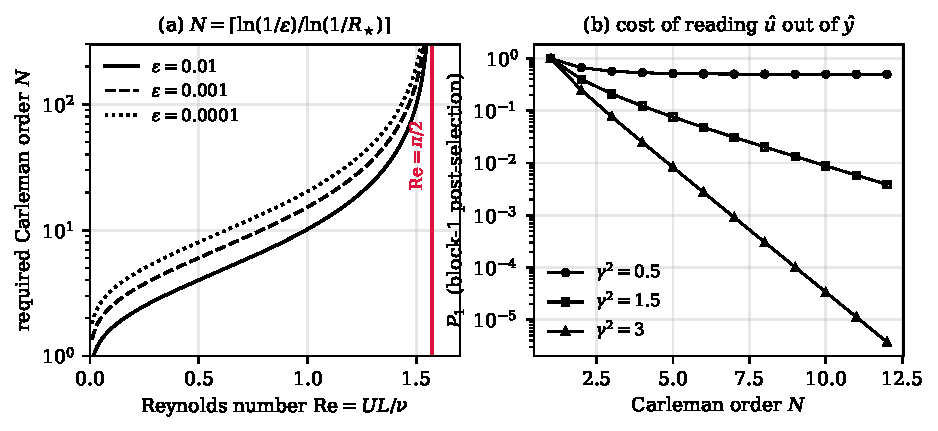
\includegraphics[width=\textwidth]{fig_carleman.pdf}
\caption{(a) Carleman order $N$ required by \eqref{eq:Nreq} to reach relative
error $\epsilon$, using the sharpened ratio $R_\star=2\Rey/\pi$ of
\eqref{eq:Rstar}.  Beyond $\Rey=\pi/2$ (red line) the series has no proven
convergence regime and no finite $N$ suffices.  (b) The block-1 post-selection
probability $P_1$ of Eq.~\eqref{eq:P1}, which decays geometrically in $N$ unless
the state is rescaled so that $\gamma=\norm{\uvec}_2<1$.}
\label{fig:carleman}
\end{figure}

\begin{remark}[Rescaling does not help]
\label{rem:rescale}
A natural thought is to rescale $\uvec\to\uvec/\Gamma$ to shrink $\norm{\uvec_0}$.
But \eqref{eq:quadode} is then satisfied with $\Ftwo\to\Gamma\Ftwo$, so the
product $\norm{\uvec_0}\norm{\Ftwo}$ in \eqref{eq:Rdef} is unchanged: $R$ is
invariant under rescaling.  This is worth internalising --- the constraint
\eqref{eq:Rstar} is physical, not a normalisation artefact.  (Rescaling
\emph{does} help with a different problem, the block-1 readout of
Section~\ref{sec:P1}.)
\end{remark}

\begin{remark}[Short-time bounds]
For non-dissipative problems (e.g.\ the Korteweg--de~Vries equation, where
$\Fone$ is skew-symmetric and $\mathrm{Re}\,\mu_1=0$ exactly, so $R=\infty$),
criterion \eqref{eq:Rdef} is vacuous and one must use finite-horizon bounds of
the form $\varepsilon_{\rm CL}\lesssim\norm{\uvec_0}(T/\tau_{\rm nl})^N$ with
$\tau_{\rm nl}=\norm{\partial_xu}_\infty^{-1}$ the nonlinear time scale
\cite{Wu2025}.  These converge only for $T<\tau_{\rm nl}$, roughly one eddy
turnover.  Restarting is not an option, because restarting requires re-preparing
an amplitude encoding of $\hat\uvec(T)$, which requires tomography.
\end{remark}

\subsection{Time discretisation error}
\label{sec:t-err}

Backward Euler is first-order accurate.  For the linear system
$\dot\yvec=\Amat\yvec$ the global error after time $T$ is (Appendix~\ref{app:fd})
\begin{equation}
\varepsilon_{\rm t}\ \simeq\ \tfrac12\,\Delta t\,T\,\norm{\Amat}^{2}\norm{\yvec},
\qquad\Longrightarrow\qquad
\Delta t=\frac{2\,\epsilon_{\rm t}}{T\norm{\Amat}^{2}},
\quad
m=\frac{T}{\Delta t}=\frac{T^{2}\norm{\Amat}^{2}}{2\,\epsilon_{\rm t}} .
\label{eq:dtreq}
\end{equation}
From \eqref{eq:Ajj}--\eqref{eq:Ajj1}, each block is a sum of $j\le N$ terms, so
\begin{equation}
\norm{\Amat}\ \le\ N\max\bigl(\norm{\Fone},\norm{\Ftwo}\norm{\uvec}\bigr)
= N\,\Lambda_{\Amat},
\qquad
\Lambda_{\Amat}:=\max\Bigl(\frac{4\nu}{\Delta x^{2}},\ \frac{U}{\sqrt2\,\Delta x}\Bigr).
\label{eq:normA}
\end{equation}
Whenever the grid resolves the viscous layer, $\Delta x\lesssim\delta_{\rm v}=\nu/U$, the
diffusive entry dominates and $\Lambda_{\Amat}\simeq4\nu/\Delta x^2 = 4n_x^2/(\Rey L^2)$.
Substituting into \eqref{eq:dtreq} gives $m=\Oh(N^2n_x^4/(\Rey^2\epsilon_{\rm t}))$,
i.e.\ $m=\Oh(\epsilon^{-3})$ once $n_x\propto\epsilon^{-1/2}$.  This is
unacceptably steep and is a defect of first-order stepping, not of the quantum
algorithm.  Replacing backward Euler by a high-order scheme --- the truncated
Taylor or linear-multistep encodings of \cite{Berry2014,Berry2017} --- gives
instead
\begin{equation}
\boxed{\ m=\Oh\!\Bigl(\norm{\Amat}\,T\,
\frac{\log(1/\epsilon_{\rm t})}{\log\log(1/\epsilon_{\rm t})}\Bigr)
=\Ot\!\Bigl(\frac{N\,n_x^{2}\,T}{\Rey}\Bigr),}
\label{eq:mreq}
\end{equation}
which we adopt for all asymptotic statements below.  We flag this as a
recommended modification to the pathway of \cite{Setty2026}: the change is
purely classical (a different sparse matrix to block-encode) and costs nothing
in qubits.

\subsection{Algorithmic errors and why they are amplified}
\label{sec:alg-err}

The errors in the middle group of Table~\ref{tab:errors} enter differently from
the discretisation errors, because they perturb the linear system rather than
the model.  If the block encoding realises $\Lmat+\delta\Lmat$ instead of
$\Lmat$, and the oracle prepares $\ket{b}+\ket{\delta b}$, then standard
perturbation theory (Appendix~\ref{app:pert}, Lemma~\ref{lem:pert}) gives
\begin{equation}
\frac{\norm{\delta\yvec}}{\norm{\yvec}}
\ \le\ \frac{\kQ}{1-\kQ\norm{\delta\Lmat}/\norm{\Lmat}}
\left(\frac{\norm{\delta\Lmat}}{\norm{\Lmat}}+\frac{\norm{\delta b}}{\norm{b}}\right)
\ \approx\ \kQ\left(\epsilon_{\rm BE}+\epsilon_b\right),
\label{eq:amplify}
\end{equation}
and the same factor multiplies the polynomial-approximation error
$\epsilon_{\rm inv}$ and the phase-synthesis error $\epsilon_\phi$.  The
practical consequence is that these four quantities must be controlled to
$\epsilon/\kQ$ rather than $\epsilon$, which adds a $\log\kQ$ to the polynomial
degree \eqref{eq:degree} and to the arithmetic precision of the block encoding.

One error in this group behaves qualitatively differently.  The polynomial
$\mathrm{Poly}(\sigma)$ approximates $1/\sigma$ only on $[1/\kappa,1]$; any
genuine singular value of $\Lmat^\dagger/\alpha$ \emph{below} the design cut-off
is not inverted but suppressed.  This is not a small perturbation --- it deletes
a spectral component --- so $\kappa$ must be chosen with
$1/\kappa\le\sigma_{\min}$ guaranteed, not merely likely.  Reference
\cite{Setty2026} handles this correctly by estimating $\sigma_{\min}$
classically first (its §2), and by choosing $\kappa$ conservatively; note this is
the reason its $\kappa=8$ exceeds our computed $\kQ=5.46$.

\subsection{Statistical error}
\label{sec:stat-err}

Finally, the output is a quantum state, and every number extracted from it
carries shot noise $\Oh(M_{\rm shot}^{-1/2})$ where $M_{\rm shot}$ is the number
of repetitions.  How many repetitions are needed depends entirely on what is
being asked for, and is quantified in Section~\ref{sec:samples}.

\subsection{Budget allocation}

We allocate the total budget \eqref{eq:epsdef} equally across the five groups,
$\varepsilon_\bullet=\epsilon/5$, which is optimal up to constants because each
cost depends only logarithmically or polynomially on its own tolerance.  This
fixes
\begin{equation}
n_x\gtrsim\max\!\left(\tfrac12\Rey,\ \sqrt{5C_{\rm sp}/\epsilon}\right),
\quad
N=\left\lceil\frac{\ln(5/\epsilon)}{\ln(\pi/2\Rey)}\right\rceil,
\quad
m=\Ot\!\left(\frac{Nn_x^2T}{\Rey}\right),
\quad
\epsilon_{\rm inv}=\epsilon_{\rm BE}=\frac{\epsilon}{5\kQ}.
\label{eq:allocation}
\end{equation}

%=====================================================================
\section{Resource estimates}
\label{sec:resources}
%=====================================================================

\subsection{Qubit count}
\label{sec:qubits}

The register structure of \cite[Fig.~2]{Setty2026} is: one QSP qubit carrying
the phase sequence; a flag register of $m_{\rm flag}$ qubits (the data qubits of
the block encoding plus one ``delete'' qubit); and a matrix register of $q_M$
qubits holding $\ket{b}$ and the encoded matrix.  Hence
\begin{equation}
\boxed{\
\#\text{qubits} = \underbrace{q_M}_{\lceil\log_2 D\rceil}
+\underbrace{m_{\rm flag}}_{\lceil\log_2 n_{\rm data}\rceil+1}
+\underbrace{1}_{\rm QSP}
+\underbrace{\Oh(1)}_{\text{amplitude amplification}} }
\label{eq:qubits}
\end{equation}
with, from \eqref{eq:Dim} and writing $q=\log_2 n_x$,
\begin{equation}
q_M=\bigl\lceil\log_2 D\bigr\rceil\simeq N q
= N\log_2 n_x .
\label{eq:qM}
\end{equation}
For the reference instance, $q_M=\lceil\log_2 30\rceil=5$,
$m_{\rm flag}=\lceil\log_2 14\rceil+1=5$, total $5+5+1=11$, matching
\cite[Table~4]{Setty2026} exactly.

Equation~\eqref{eq:qM} is the pathway's one unambiguous success: the state
register is \emph{logarithmic} in the grid size and \emph{linear} in the
Carleman order, so a $2^{10}$-point grid at $N=6$ needs only $60$ matrix qubits
where a classical solver would store $10^{18}$ numbers.  Everything that follows
is the story of how that compression is paid for elsewhere.

\subsection{Subnormalisation and the effective condition number}
\label{sec:kappa}

\paragraph{Which condition number?}  Reference~\cite{Setty2026} writes $\kappa$
for ``the condition number'' without specifying whether it refers to $\Lmat$ or
to the subnormalised $\Lmat/\alpha$.  The distinction matters, because the
polynomial in \eqref{eq:degree} must invert the singular values of
$\Lmat^\dagger/\alpha$, which are $\sigma_k(\Lmat)/\alpha$.  The cut-off must
therefore satisfy $1/\kappa\le\sigma_{\min}(\Lmat)/\alpha$, i.e.
\begin{equation}
\boxed{\ \kQ\ :=\ \frac{\alpha}{\sigma_{\min}(\Lmat)}\ }
\qquad\text{not}\qquad
\frac{\sigma_{\max}(\Lmat)}{\sigma_{\min}(\Lmat)}.
\label{eq:kQ}
\end{equation}
The two coincide only if $\alpha$ is chosen equal to $\sigma_{\max}$, which is
not achievable for a sparse-oracle block encoding.  Table~\ref{tab:kappa}
settles the question empirically against the three worked examples of
\cite{Setty2026}: $\kQ$ tracks the design values, the classical condition number
does not.

\begin{table}[htbp]
\centering
\caption{Which condition number sets the QSVT degree?  Reconstructed from the
three examples of \cite{Setty2026}.  The design value $\kappa$ is what the paper
used to synthesise the phases.  $\kQ=\alpha/\sigma_{\min}$ tracks it to within
the deliberate safety margin; $\sigma_{\max}/\sigma_{\min}$ does not.}
\label{tab:kappa}
\small
\begin{tabular}{@{}lcccccc@{}}
\toprule
Instance & $\alpha$ & $\sigma_{\max}$ & $\sigma_{\min}$
& $\dfrac{\sigma_{\max}}{\sigma_{\min}}$ & $\kQ=\dfrac{\alpha}{\sigma_{\min}}$
& design $\kappa$ of \cite{Setty2026}\\
\midrule
Burgers, §4.3 ($n_x=5$, $N=2$)   & $4.76$ & $1.37$ & $0.872$ & $1.57$ & $5.46$ & $8$\\
Heat, §4.2 ($q_M=3$)             & $4.84$ & $3.57$ & $1.014$ & $3.52$ & $4.77$ & $8$\\
Heat, §4.2 ($q_M=4$)             & $4.84$ & $3.57$ & $1.000$ & $3.57$ & $4.84$ & $12$\\
\bottomrule
\end{tabular}
\end{table}

\paragraph{Computing $\alpha$ in closed form.}  For the coherent-permutation
block encoding of \cite{Setty2025BE} used in \cite{Setty2026}, the
subnormalisation is the $\ell^1$ norm of the \emph{data vector} --- the list of
distinct matrix values, each tagged with the diagonal offset (row minus column)
on which it repeats:
\begin{equation}
\alpha=\norm{v_{\rm data}}_1=\sum_i\abs{\psi_i},
\qquad
n_{\rm data}=\#\{(\text{value},\ \text{offset})\ \text{pairs of }\Lmat\}.
\end{equation}
Counting these pairs for $\Lmat=\Id-\Delta t\Amat$ using
\eqref{eq:Ajj}--\eqref{eq:Ajj1}:
\begin{itemize}[nosep,leftmargin=*]
\item \emph{Diagonals.}  Block $j$ has diagonal entry $1+2j\lambda_{\rm diff}$
(each of the $j$ copies of $\Fone$ contributes $-2\lambda_1\Delta t$), giving $N$
distinct values summing to $N+N(N+1)\lambda_{\rm diff}$.
\item \emph{Off-diagonal $\Fone$ entries.}  In block $j$ the copies of $\Fone$
sit at offsets $\pm n_x^{v}$, $v=0,\dots,j-1$.  Across all blocks these coincide,
leaving $2N$ distinct offsets, each of magnitude $\lambda_{\rm diff}$.
\item \emph{$\Ftwo$ entries.}  These live in the \emph{rectangular} blocks
$A^j_{j+1}$, whose entries do \emph{not} lie on constant diagonals of the square
embedding: the offset varies from row to row.  This produces
$\Theta(n_x^{\,N-1})$ distinct pairs, each of magnitude $\lambda_{\rm cfl}/2$.
\end{itemize}
Hence
\begin{equation}
\boxed{\
n_{\rm data}=N+2N+\Theta\!\left(n_x^{\,N-1}\right),
\qquad
\alpha=\underbrace{N+N(N+1)\lambda_{\rm diff}+2N\lambda_{\rm diff}}_{\text{linear part}}
+\underbrace{\Theta\!\left(n_x^{\,N-1}\right)\frac{\lambda_{\rm cfl}}{2}}_{\text{nonlinear part}} .}
\label{eq:alpha}
\end{equation}
For $N=2$ the last count is exactly $2(n_x-1)$, giving
$n_{\rm data}=3N+2(n_x-1)$, which for $n_x=5$, $N=2$ evaluates to $14$ --- the
number of data elements in \cite[Table~3]{Setty2026}.
Equation~\eqref{eq:ndata} below records the exact $N=2$ formula.  The $\alpha$
formula is verified to be \emph{exact} against direct construction of the
matrices over a range of $\Delta t$ spanning three orders of magnitude
(Appendix~\ref{app:numerics}).
\begin{equation}
n_{\rm data}\big|_{N=2}=3N+2(n_x-1)=6+2(n_x-1).
\label{eq:ndata}
\end{equation}

\paragraph{The bad news.}  Because $\alpha$ enters $\kQ$ and hence the
polynomial degree linearly, \eqref{eq:alpha} says
\begin{equation}
\kQ\ \simeq\ \alpha\ \simeq\ n_x^{\,N-1}\lambda_{\rm cfl}
\qquad(\text{coherent-permutation block encoding}),
\label{eq:kQbad}
\end{equation}
where we used $\sigma_{\min}(\Lmat)=\Oh(1)$, which holds because $\Amat$ has
eigenvalues with non-positive real part so $\Lmat=\Id-\Delta t\Amat$ has
eigenvalues of modulus $\ge1$.  This is polynomial in the grid size and
\emph{exponential in the Carleman order} --- precisely the scaling that the
logarithmic qubit count \eqref{eq:qM} was supposed to avoid.
Figure~\ref{fig:alpha} shows the measured growth.

\subsection{Two block encodings, and why the choice dominates everything}
\label{sec:two-be}

The scaling \eqref{eq:kQbad} is a property of the \emph{construction}, not of
block encoding as such.  The coherent-permutation scheme of \cite{Setty2025BE}
loads all distinct matrix values into a data register and permutes them onto
constant diagonals; it is excellent for Toeplitz-like matrices from finite
differences, which is what it was designed for, and poorly matched to the
rectangular Kronecker blocks $A^j_{j+1}$ of the Carleman matrix.

The standard alternative is the \emph{sparse-access oracle} block encoding
(Appendix~\ref{app:be}).  It requires two oracles: $O_{\rm loc}$, which given a
row index and a counter $\ell\le s$ returns the column index of the $\ell$-th
nonzero; and $O_{\Lmat}$, which returns the corresponding value.  Both are
computed \emph{arithmetically} from the closed-form structure
\eqref{eq:Ajj}--\eqref{eq:Ajj1} rather than looked up in a table, and the
subnormalisation is
\begin{equation}
\alpha_{\rm sp}=s\,\norm{\Lmat}_{\max},
\qquad
s=\max_{\rm rows}\#\{\text{nonzeros}\}=4N-3,
\qquad
\norm{\Lmat}_{\max}=1+2N\lambda_{\rm diff},
\label{eq:alphasp}
\end{equation}
so that
\begin{equation}
\boxed{\ \alpha_{\rm sp}=(4N-3)(1+2N\lambda_{\rm diff})=\Oh\!\left(N^{2}\lambda_{\rm diff}\right),}
\label{eq:kQgood}
\end{equation}
\emph{independent of $n_x$ except through the diffusion number}.  The row
sparsity $s=4N-3$ is verified numerically (Appendix~\ref{app:numerics}): each row
of $A^j_j$ has $2j+1$ nonzeros and each row of $A^j_{j+1}$ has $2j$, but the
maxima are not attained simultaneously.  Table~\ref{tab:BEcompare} quantifies
the gap.

\begin{table}[htbp]
\centering
\caption{Subnormalisation for the two block-encoding routes ($\nu=0.01$,
$\Delta t=0.1$).  $\alpha_{\rm cp}$ is the coherent-permutation value of
\cite{Setty2026}, computed exactly from the assembled matrix;
$\alpha_{\rm sp}=s\norm{\Lmat}_{\max}$ is the sparse-oracle value.  The final
column is the factor by which the published construction inflates the QSVT
degree.}
\label{tab:BEcompare}
\small
\begin{tabular}{@{}ccccccc@{}}
\toprule
$n_x$ & $N$ & $D$ & $n_{\rm data}$ & $\alpha_{\rm cp}$ & $\alpha_{\rm sp}$ & ratio\\
\midrule
$5$ & $2$ & $30$   & $14$  & $4.76$   & $5.72$  & $0.83$\\
$7$ & $2$ & $56$   & $18$  & $7.44$   & $6.28$  & $1.18$\\
$9$ & $2$ & $90$   & $22$  & $11.00$  & $7.00$  & $1.57$\\
$15$& $2$ & $240$  & $34$  & $26.96$  & $10.12$ & $2.66$\\
$21$& $2$ & $462$  & $46$  & $50.84$  & $13.24$ & $3.84$\\
\midrule
$5$ & $3$ & $155$  & $65$  & $20.45$  & $10.94$ & $1.87$\\
$7$ & $3$ & $399$  & $117$ & $47.35$  & $12.46$ & $3.80$\\
$9$ & $3$ & $819$  & $185$ & $92.80$  & $14.40$ & $6.44$\\
$15$& $3$ & $3615$ & $485$ & $388.41$ & $22.82$ & $17.02$\\
\bottomrule
\end{tabular}
\end{table}

\begin{figure}[htbp]
\centering
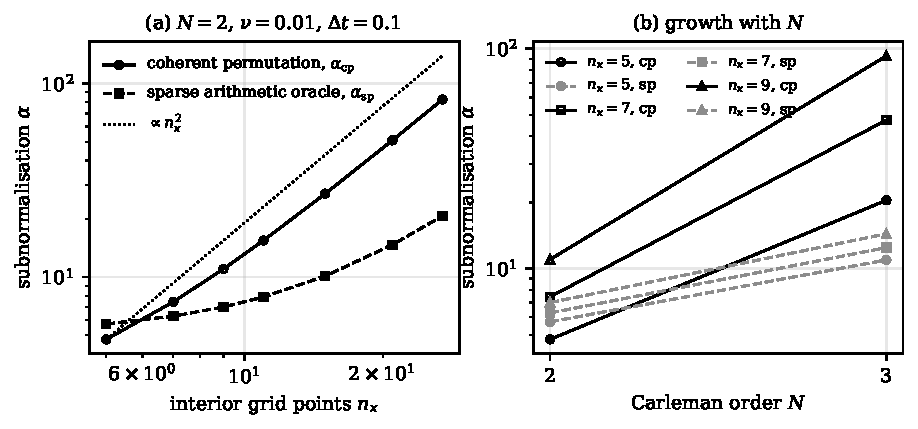
\includegraphics[width=\textwidth]{fig_alpha.pdf}
\caption{Growth of the block-encoding subnormalisation $\alpha$, which sets the
QSVT polynomial degree through $\kQ=\alpha/\sigma_{\min}$.  (a) With grid size at
fixed Carleman order $N=2$: the coherent-permutation construction of
\cite{Setty2026} (circles) grows as $n_x^{N-1}\lambda_{\rm cfl}\propto n_x^2$
here because $\lambda_{\rm cfl}\propto n_x$ at fixed $\Delta t$, while the
sparse arithmetic oracle (squares) stays nearly flat.  (b) With Carleman order:
the gap widens rapidly, reaching a factor $17$ at $n_x=15,N=3$.}
\label{fig:alpha}
\end{figure}

\paragraph{The trade.}  The sparse oracle buys a much smaller $\alpha$ at the
cost of quantum arithmetic: $O_{\rm loc}$ must add and compare $q_M$-bit
integers, which needs ripple-carry adders of depth $\Oh(q_M)$ and $\Oh(q_M)$
ancillas, and $O_{\Lmat}$ must synthesise a rotation angle from the entry value.
The coherent-permutation route avoids arithmetic entirely but pays $\Oh(n_{\rm data})$
in both gate count and subnormalisation.  For the small instances in
\cite{Setty2026} the coherent-permutation route is genuinely better
(row 1 of Table~\ref{tab:BEcompare}); asymptotically it is not.  \textbf{We
recommend the sparse-oracle route for any scaling study, and all asymptotic
statements below assume it.}

\subsection{Polynomial degree}
\label{sec:degree}

With $\kQ$ from \eqref{eq:kQ} and the accuracy allocation
$\epsilon_{\rm inv}=\epsilon/(5\kQ)$ from \eqref{eq:allocation}, the Chebyshev
construction of \cite[Appendix~B]{Setty2026} (reproduced in
Appendix~\ref{app:qsvt}) gives
\begin{equation}
b_{\rm ch}=\kQ^{2}\log(\kQ/\epsilon_{\rm inv}),
\qquad
\boxed{\ d=\bigl\lceil\sqrt{b_{\rm ch}}\,\log(4b_{\rm ch}/\epsilon_{\rm inv})\bigr\rceil
=\Oh\!\bigl(\kQ\log(\kQ/\epsilon)\bigr).}
\label{eq:d}
\end{equation}

\begin{remark}[A reproducibility gap in the source]
The pairs $(\kappa,d)$ reported in \cite{Setty2026} are
$(4,117)$, $(8,559)$ and $(12,1275)$.  Fitting a power law gives $d\propto\kappa^{2.1}$,
whereas \eqref{eq:d} predicts $d\propto\kappa$ up to logarithms.  The
discrepancy is resolved by noting that $d$ also depends on
$\epsilon_{\rm inv}$, which is not stated: inverting \eqref{eq:d} shows the
three cases correspond to $\epsilon_{\rm inv}\approx10^{-2}$, $10^{-5}$ and
$10^{-5}$ respectively.  We record this because it means the published degrees
cannot be compared with each other directly, and because any future scaling
study should report $\epsilon_{\rm inv}$ alongside $\kappa$.
\end{remark}

\subsection{Circuit depth}
\label{sec:depth}

The QSVT circuit \cite[Fig.~2]{Setty2026} interleaves $d$ applications of
$U_{\Lmat}$ (alternating with $U_{\Lmat}^\dagger$) with $d+1$
projector-controlled phase shifts $\Pi_{\phi_i}$, each a multi-controlled
rotation on the flag register.  Therefore
\begin{equation}
D_{\rm QSVT}\ \simeq\ d\,\bigl(D_{\rm BE}+D_{\Pi}\bigr),
\label{eq:depthmodel}
\end{equation}
where $D_{\rm BE}$ and $D_\Pi$ are the two-qubit depths of one block encoding
and one phase shift.  We calibrate both against the four instances in
\cite[Tables~1,2,4]{Setty2026}.  Fitting the heavy-hex numbers gives
\begin{equation}
D_{\rm BE}\ \simeq\ c_{\rm BE}\,n_{\rm data}\,q_M^{2},
\qquad
D_{\Pi}\ \simeq\ c_{\Pi}\,m_{\rm flag}^{2},
\qquad
c_{\rm BE}\approx10,\quad c_{\Pi}\approx15 .
\label{eq:depthfit}
\end{equation}
The $q_M^2$ and $m_{\rm flag}^2$ scalings are not assumed: the exponent on
$q_M$ is extracted from the two heat-equation rows, which differ only in $q_M$,
via $\log(550/311)/\log(4/3)=1.98$.  Table~\ref{tab:depthfit} and
Figure~\ref{fig:depth} show the model reproduces depths spanning a factor of
$60$ to within a factor of $1.6$.

\begin{table}[htbp]
\centering
\caption{Calibration of the depth model \eqref{eq:depthmodel}--\eqref{eq:depthfit}
against the heavy-hex two-qubit depths reported in \cite{Setty2026}.
$D_\Pi^{\rm obs}$ is inferred as $D_{\rm QSVT}/d-D_{\rm BE}$.}
\label{tab:depthfit}
\small
\begin{tabular}{@{}lcccccccc@{}}
\toprule
Instance & $d$ & $q_M$ & $n_{\rm data}$ & $m_{\rm flag}$
& $D_{\rm BE}$ & $D_\Pi^{\rm obs}$ & $D_{\rm QSVT}$ & model\\
\midrule
Complex tridiagonal & $117$  & $3$ & $6$  & $4$ & $283$  & $204$ & $57$K  & $91$K\\
Heat, $q_M=3$       & $559$  & $3$ & $4$  & $3$ & $311$  & $151$ & $258$K & $277$K\\
Heat, $q_M=4$       & $1275$ & $4$ & $4$  & $3$ & $550$  & $158$ & $903$K & $988$K\\
Burgers             & $559$  & $5$ & $14$ & $5$ & $5687$ & $395$ & $3.4$M & $2.2$M\\
\bottomrule
\end{tabular}
\end{table}

\begin{figure}[htbp]
\centering
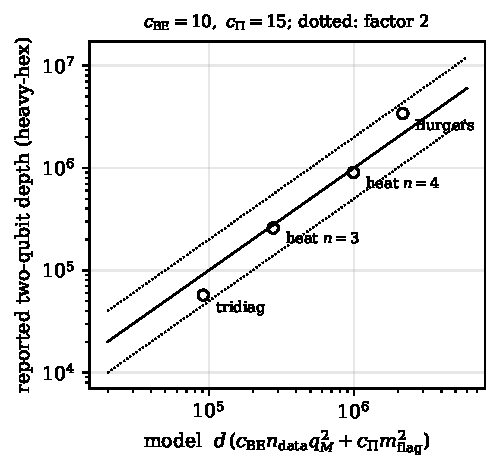
\includegraphics[width=0.46\textwidth]{fig_depth.pdf}
\caption{The depth model \eqref{eq:depthmodel}--\eqref{eq:depthfit} against the
four instances reported in \cite{Setty2026}.  Solid line: perfect agreement;
dotted lines: a factor of two either way.}
\label{fig:depth}
\end{figure}

For the sparse-oracle route, $D_{\rm BE}$ is instead dominated by the arithmetic
in $O_{\rm loc}$: computing a column index requires $\Oh(1)$ additions and
comparisons of $q_M$-bit integers, each of two-qubit depth $\Oh(q_M)$, plus a
value-dependent rotation, so
\begin{equation}
D_{\rm BE}^{\rm sp}=\Oh\!\left(s\,q_M+q_M^{2}\right)
=\Oh\!\left(N q_M+q_M^{2}\right).
\label{eq:BEsp}
\end{equation}

\subsection{Success probability and the Carleman-block penalty}
\label{sec:P1}
\label{sec:success}

\paragraph{QSVT post-selection.}  Substituting $\beta=1/(2\kQ)$ into
\eqref{eq:ps} and defining the \emph{achieved} inverse norm
$\kappa_{\rm eff}:=\lVert(\Lmat^\dagger/\alpha)^{-1}\ket{b}\rVert$, which lies in
$[1,\kQ]$,
\begin{equation}
\boxed{\ p_s=\left(\frac{\kappa_{\rm eff}}{2\,\kQ^{\rm design}}\right)^{2}
\ \in\ \left[\frac{1}{4(\kQ^{\rm design})^2},\ \frac14\right].}
\label{eq:psmodel}
\end{equation}
The upper bound $1/4$ is reached when the design cut-off is tight.  For the
reference instance $\kappa_{\rm eff}=4.83$ and $\kQ^{\rm design}=8$, giving
$p_s=0.0911$ against the reported $0.0865$ --- agreement to $5\%$, which is the
strongest single validation of our reconstruction.  It also shows where the
factor of three below the ideal $1/4$ comes from: the conservative choice
$\kappa=8$ against an actual requirement of $5.5$.

\paragraph{The Carleman block penalty.}  The solution state is the normalised
Carleman vector $\ket{\hat y}=\ket{(\hat y_1;\dots;\hat y_N)}$, but the physical
field is only $\hat y_1$.  Since $\norm{\hat y_j}=\norm{\uvec}^j$, writing
$\gamma:=\norm{\uvec}_2$ the probability of finding the block register in state
``$1$'' is
\begin{equation}
\boxed{\ P_1=\frac{\norm{\uvec}^{2}}{\sum_{j=1}^{N}\norm{\uvec}^{2j}}
=\frac{\gamma^{2}}{\sum_{j=1}^{N}\gamma^{2j}}
=\begin{cases}
\dfrac{1-\gamma^{2}}{1-\gamma^{2N}}, & \gamma<1,\\[3mm]
\dfrac{\gamma^{-2(N-1)}(1-\gamma^{-2})}{1-\gamma^{-2N}}, & \gamma>1.
\end{cases}}
\label{eq:P1}
\end{equation}
This is a genuine and, to our knowledge, undiscussed cost.  If $\gamma>1$ the
Carleman vector is dominated by its \emph{highest} block and $P_1$ decays
geometrically, as $\gamma^{-2(N-1)}$.  For the reference instance
$\gamma^2=\norm{\uvec_0}^2=3$, giving $P_1=1/4$ at $N=2$ but $P_1=2.8\times10^{-3}$
at $N=6$ (Figure~\ref{fig:carleman}(b)).

The fix is to rescale $\uvec\to\uvec/\Gamma$ with $\Gamma>\gamma$, which by
Remark~\ref{rem:rescale} leaves the Carleman convergence ratio $R$ untouched and
makes $P_1=1-\gamma^2/\Gamma^2=\Oh(1)$.  \textbf{We recommend normalising the
discrete initial data to $\norm{\uvec_0}_2<1$ before building the Carleman
matrix}; it is free and it removes an exponential-in-$N$ overhead.

\subsection{The sequential-stepping obstruction, and the dilated system}
\label{sec:sequential}

Reference~\cite{Setty2026} advances one implicit step at a time: it solves
$\Lmat\yvec^{k+1}=\yvec^{k}$ for $k=0,\dots,m-1$ with $m=T/\Delta t=3$.  In a
state-vector simulation this is unproblematic, because the classical simulator
can read out $\yvec^{k+1}$ and re-prepare it.  On hardware it is not.

\begin{proposition}[Sequential solves compound]
\label{prop:seq}
Let each step succeed on post-selection with probability $p_s$.  Then producing
$\ket{\yvec^{m}}$ by chaining $m$ QSVT solves requires
$\Oh(p_s^{-m/2})$ applications of the chain even with optimal amplitude
amplification.
\end{proposition}

\begin{proof}[Sketch]
Amplitude amplification of a state $U\ket{0}=\sqrt{p}\ket{\rm good}+\dots$ to
near-unit success requires $\Oh(p^{-1/2})$ applications of $U$, $U^\dagger$ and
the reflection $2\ket{0}\!\bra{0}-\Id$.  To amplify step $k$ alone one needs the
reflection about \emph{its} input state $U_{k-1}\cdots U_1\ket{0}$, which
requires re-running the entire preceding chain.  The costs therefore multiply
rather than add, giving $\prod_{k}\Oh(p_s^{-1/2})=\Oh(p_s^{-m/2})$.  Amplifying
the whole chain at once gives the same count, since
$p_{\rm total}=p_s^{m}$.
\end{proof}

For the reference instance ($p_s=0.087$, $m=3$) this is a factor of $38$ --- an
inconvenience.  At $m=300$ it is $10^{159}$.  Sequential stepping is therefore
not merely inefficient but fatal, and any scaling claim must use the alternative.

\paragraph{The history-state formulation.}  Encode all time levels at once
\cite{Berry2014,Berry2017,Liu2021}.  Introduce a time register of dimension
$m+n_{\rm pad}+1$, where $n_{\rm pad}$ is a number of padding levels, and define the
dilated matrix
\begin{equation}
\mathcal{L}=
\begin{pmatrix}
\Id & & & & & \\
-\Id & \Lmat & & & & \\
 & \ddots & \ddots & & & \\
 & & -\Id & \Lmat & & \\
 & & & -\Id & \Id & \\
 & & & & \ddots & \ddots \\
 & & & & & -\Id & \Id
\end{pmatrix}
\in\R^{(m+n_{\rm pad}+1)D\times(m+n_{\rm pad}+1)D},
\label{eq:dilated}
\end{equation}
whose first row block imposes $\yvec^0=\yvec_{\rm in}$, whose next $m$ row blocks
impose the time stepping \eqref{eq:implicit}, and whose last $n_{\rm pad}$ row blocks
simply copy $\yvec^m$ so as to raise its share of the total amplitude.  Solving
$\mathcal{L}\bm{Y}=(\yvec_{\rm in};0;\dots;0)$ in one QSVT call produces the
\emph{history state}
$\ket{\bm Y}\propto\sum_{k}\ket{k}\otimes\ket{\yvec^{k}}$, from which
$\ket{\yvec^m}$ is obtained by measuring the time register in the padding range.

\begin{proposition}[Condition number of the dilated system]
\label{prop:dilkappa}
If all eigenvalues of $\Amat$ have non-positive real part, then
\begin{equation}
\kappa(\mathcal{L})\ \le\ \kappa_V(\Amat)\,(m+n_{\rm pad}+1)\,\bigl(2+\Delta t\norm{\Amat}\bigr),
\label{eq:dilkappa}
\end{equation}
where $\kappa_V(\Amat)$ is the eigenvector condition number, i.e.\ the condition
number of the matrix $V$ diagonalising $\Amat=V\Sigma V^{-1}$.
\end{proposition}

\begin{proof}
$\norm{\mathcal{L}}\le1+\norm{\Lmat}\le2+\Delta t\norm{\Amat}$ by the triangle
inequality on the two nonzero block-diagonals.  For the inverse, block
forward-substitution gives
$[\mathcal{L}^{-1}]_{k,j}=\Lmat^{-(k-j)}$ for $k\ge j$ and $0$ otherwise, so
$\norm{\mathcal{L}^{-1}}\le\sum_{k=0}^{m+n_{\rm pad}}\norm{\Lmat^{-k}}$.  Diagonalising
$\Amat=V\Sigma V^{-1}$ gives
$\norm{\Lmat^{-k}}\le\kappa_V\max_i\abs{1-\Delta t\mu_i}^{-k}\le\kappa_V$,
since $\mathrm{Re}\,\mu_i\le0$ implies $\abs{1-\Delta t\mu_i}\ge1$.  Summing the
$m+n_{\rm pad}+1$ terms gives the claim.
\end{proof}

\begin{corollary}[The key cancellation]
\label{cor:cancel}
With $n_{\rm pad}=m$, and using $\norm{\Amat}\simeq4N\nu/\Delta x^2$ from
\eqref{eq:normA} so that $\Delta t\norm{\Amat}\simeq4N\lambda_{\rm diff}$,
\begin{equation}
\kappa(\mathcal{L})=\Oh\!\bigl(\kappa_V\,m\,N\lambda_{\rm diff}\bigr)
=\Oh\!\left(\kappa_V\,N\,\frac{T}{\Delta t}\cdot\frac{\Delta t}{\Rey\Delta x^{2}}\right)
=\boxed{\ \Oh\!\left(\frac{\kappa_V\,N\,T\,n_x^{2}}{\Rey\,L^{2}}\right)}
\label{eq:dilkappa2}
\end{equation}
which is \emph{independent of the time step $\Delta t$}.
\end{corollary}

Corollary~\ref{cor:cancel} is what makes the pathway analysable at all: the
factors of $\Delta t$ in the step count $m=T/\Delta t$ and in the diffusion
number $\lambda_{\rm diff}\propto\Delta t$ cancel exactly.  Refining the time
step costs nothing in the QSVT degree; it costs only in the size of the time
register, i.e.\ $\log_2 m$ extra qubits.  The physically meaningful cost is
$Tn_x^2/\Rey$, which is the number of \emph{diffusive} time scales resolved.

\subsection{Success probability of the assembled algorithm}

Collecting the three post-selections --- QSVT flags, time register, and Carleman
block --- and writing $g:=\max_k\norm{\yvec^k}/\norm{\yvec^m}$ for the norm
decay of the trajectory,
\begin{equation}
\boxed{\
p_{\rm tot}
=\underbrace{p_s}_{\le1/4}\times
\underbrace{\frac{n_{\rm pad}}{m+n_{\rm pad}}\cdot\frac{1}{g^{2}}}_{\text{time register}}\times
\underbrace{P_1}_{\text{Eq.~}\eqref{eq:P1}} }
\label{eq:ptot}
\end{equation}
and with amplitude amplification the query cost multiplies by
$\Oh(p_{\rm tot}^{-1/2})$.  With the recommendations of this section
($n_{\rm pad}=m$, $\norm{\uvec_0}_2<1$, tight $\kappa$) all three factors are $\Oh(1)$ and
$p_{\rm tot}^{-1/2}=\Oh(1)$; without them, each can be exponentially small.

\subsection{Sample complexity}
\label{sec:samples}

What must be measured, and how often, depends entirely on the deliverable.  We
distinguish three regimes; $M_{\rm shot}$ denotes the number of circuit
repetitions.

\begin{enumerate}[leftmargin=*]
\item \textbf{The state itself}, e.g.\ as input to a further quantum routine.
Then $M_{\rm shot}=\Oh(p_{\rm tot}^{-1/2})$ coherent repetitions with amplitude
amplification, i.e.\ $\Oh(1)$ with the recommendations above.

\item \textbf{A scalar observable} $\langle\mathcal{M}\rangle=\bra{\hat u}\mathcal{M}\ket{\hat u}$
(drag, energy, a Fourier mode) to additive accuracy $\epsilon_{\rm obs}$.
Naive sampling needs $M_{\rm shot}=\Oh(\epsilon_{\rm obs}^{-2}p_{\rm tot}^{-1})$;
amplitude estimation (Appendix~\ref{app:aa}) reduces this to
\begin{equation}
M_{\rm shot}=\Oh\!\left(\frac{1}{\epsilon_{\rm obs}\sqrt{p_{\rm tot}}}\right).
\end{equation}
The normalisation $\norm{\hat\uvec(T)}_2$, which the amplitude encoding does
\emph{not} carry, is obtained from the same estimator applied to the heralding
flag at cost $\Oh(\epsilon_{\rm norm}^{-1})$.

\item \textbf{The whole field}, i.e.\ all $n_x$ amplitudes to relative $\ell^2$
accuracy $\epsilon$.  Pure-state tomography requires
\begin{equation}
\boxed{\ M_{\rm shot}=\Oh\!\left(\frac{n_x}{\epsilon^{2}\sqrt{p_{\rm tot}}}\right),}
\label{eq:tomo}
\end{equation}
which is linear in the grid size and therefore destroys any exponential
advantage on its own.  This is the point \cite{Setty2026} makes in its §2 and
returns to in its discussion, and it is not avoidable: the amplitude encoding
holds $n_x$ real numbers in $\log_2 n_x$ qubits, and extracting $n_x$ numbers
takes $\Omega(n_x)$ measurements by an information-theoretic argument.
\end{enumerate}

Regime 3 is what the challenge specification nominally asks for (an amplitude
encoding of the solution), but read carefully it asks only for the \emph{state},
which is regime 1.  We flag the distinction because the two differ by a factor
of $n_x/\epsilon^2$ --- for $n_x=10^3$, $\epsilon=10^{-2}$, that is $10^7$.

\subsection{Classical pre- and post-processing}
\label{sec:classical-side}

The quantum circuit is not self-contained; three classical computations must
accompany it.

\begin{enumerate}[nosep,leftmargin=*]
\item \textbf{Estimating $\sigma_{\min}(\Lmat)$} to fix the design $\kappa$.
Reference~\cite{Setty2026} correctly notes that the $n_x^N\times n_x^N$ matrix
must never be built: for the block-bidiagonal $\Amat$ the spectrum is the union
of sums of $j$ eigenvalues of $\Fone$ (Appendix~\ref{app:spectra}), all available
in closed form from \eqref{eq:F1spec}.  Cost: $\Oh(n_x)$ time, $\Oh(1)$ memory.
For the non-normal case one may need Gershgorin bounds or a Lanczos iteration on
the \emph{structure}, still $\Oh(\mathrm{poly}(n_x,N))$.

\item \textbf{Computing the phase factors} $\vec\phi\in\R^{d+1}$.  Naive
root-finding on the Chebyshev expansion costs $\Oh(d^3)$ and loses precision;
the optimisation-based methods of \cite{Dong2021,Chao2020} achieve
$\Oh(d\,\mathrm{polylog}\,d)$ time and $\Oh(d)$ memory at machine precision.
With $d\sim10^{6}$ this is seconds, not a bottleneck --- but it \emph{is} a
classical computation whose cost grows with $\kQ$, and should be reported.

\item \textbf{Post-processing} the measurement record: negligible in regimes 1
and 2, $\Oh(n_x)$ in regime 3.
\end{enumerate}

Classical memory for the whole pipeline is $\Oh(N+d)$: the $\Oh(N)$ distinct
matrix values plus the phase list.  \emph{At no point is the $D\times D$ matrix
instantiated}, and any implementation that does so has already lost.

\subsection{Assembled scaling}
\label{sec:assembled}

We now combine everything.  Assumptions, stated once: (a) sparse-oracle block
encoding, \eqref{eq:kQgood}; (b) high-order time integration, \eqref{eq:mreq};
(c) history-state formulation, \eqref{eq:dilated}; (d) initial data normalised
to $\gamma<1$; (e) $\Rey<\pi/2$ so that $N$ is finite; (f) the grid resolves the
solution, $n_x=\Theta(\epsilon^{-1/2})$.

From Corollary~\ref{cor:cancel}, $\kQ=\Oh(\kappa_V NTn_x^2/\Rey)$.  Substituting
$n_x^2=\Theta(\epsilon^{-1})$,
\begin{equation}
\kQ=\Oh\!\left(\frac{\kappa_V\,N\,T}{\Rey\,\epsilon}\right),
\qquad
d=\Ot(\kQ),
\qquad
q_M=\Theta(N\log_2 n_x)+\log_2(2m).
\end{equation}
With $D^{\rm sp}_{\rm BE}=\Oh(Nq_M+q_M^2)=\Ot(N^2\log^2 n_x)$ from
\eqref{eq:BEsp}, the sequential two-qubit depth is
\begin{equation}
\boxed{\
D_{\rm QSVT}
=\Ot\!\left(\frac{\kappa_V\,T}{\Rey\,\epsilon}\;N^{3}\log^{2}n_x\;
p_{\rm tot}^{-1/2}\right)
\ \xrightarrow[\ p_{\rm tot}=\Oh(1)\ ]{}\
\Ot\!\left(\frac{\kappa_V\,T\,N^{3}}{\Rey\,\epsilon}\right),}
\label{eq:finaldepth}
\end{equation}
with
\begin{equation}
N=\left\lceil\frac{\ln(1/\epsilon)}{\ln\bigl(\pi/(2\Rey)\bigr)}\right\rceil
=\Theta\!\left(\frac{\log(1/\epsilon)}{\log(\pi/2\Rey)}\right),
\qquad
\#\text{qubits}=\Theta\!\left(\frac{\log^{2}(1/\epsilon)}{\log(\pi/2\Rey)}\right).
\label{eq:finalqubits}
\end{equation}
Table~\ref{tab:assembled} summarises, and Table~\ref{tab:worked} evaluates a
concrete instance.

\begin{table}[htbp]
\centering
\caption{Assembled resource scaling for the QSVT pathway applied to
one-dimensional viscous Burgers, under assumptions (a)--(f) of
Section~\ref{sec:assembled}.  $\kappa_V$ is the eigenvector condition number of
the Carleman matrix (Proposition~\ref{prop:dilkappa}); it is the least
controlled quantity in the table.}
\label{tab:assembled}
\footnotesize
\begin{tabular}{@{}l>{\raggedright\arraybackslash}p{7.4cm}l@{}}
\toprule
Resource & Scaling & Driver\\
\midrule
Logical qubits & $\Theta\!\left(N\log n_x+\log m\right)
= \Theta\!\left(\log^2(1/\epsilon)/\log\tfrac{\pi}{2\Rey}\right)$ & Carleman order $\times$ grid\\
Carleman order $N$ & $\Theta\!\left(\log(1/\epsilon)\big/\log\tfrac{\pi}{2\Rey}\right)$ & diverges as $\Rey\to\pi/2$\\
Grid points $n_x$ & $\Theta\!\left(\max(\Rey,\epsilon^{-1/2})\right)$ & viscous layer, 2nd-order stencil\\
Time steps $m$ & $\Ot\!\left(TNn_x^2/\Rey\right)$ & only enters as $\log m$ qubits\\
Effective $\kQ$ & $\Oh\!\left(\kappa_V N T n_x^2/\Rey\right)=\Oh(\kappa_V NT/(\Rey\epsilon))$ & dilated system\\
Polynomial degree $d$ & $\Ot(\kQ)$ & QSVT inversion\\
Block-encoding depth & $\Oh(Nq_M+q_M^2)$ & sparse arithmetic oracle\\
\textbf{Total depth} & $\Ot\!\left(\kappa_V T N^{3}\Rey^{-1}\epsilon^{-1}\right)$ & \\
Queries to $\mathcal{U}_0$ & $\Oh(p_{\rm tot}^{-1/2})=\Oh(1)$ & amplitude amplification\\
Shots (state) & $\Oh(1)$ & \\
Shots (observable) & $\Oh(\epsilon_{\rm obs}^{-1})$ & amplitude estimation\\
Shots (full field) & $\Oh(n_x\epsilon^{-2})$ & tomography\\
Classical time & $\Ot(d)+\Oh(n_x)$ & phase synthesis, $\sigma_{\min}$\\
Classical memory & $\Oh(N+d)$ & never build the matrix\\
\bottomrule
\end{tabular}
\end{table}

\begin{table}[htbp]
\centering
\caption{A worked instance at the largest Reynolds number for which the Carleman
series provably converges.  Parameters: $\Rey=1$ (so $R_\star=2/\pi=0.637$),
$\epsilon=10^{-3}$, $T=0.3$, $n_x=2^{7}=128$, $\lambda_{\rm diff}=1$.  Depths are
logical two-qubit gates.}
\label{tab:worked}
\small
\begin{tabular}{@{}llr@{}}
\toprule
Quantity & Source & Value\\
\midrule
Carleman order $N$ & Eq.~\eqref{eq:Nreq}, $R_\star=0.637$ & $16$\\
System dimension $D$ & Eq.~\eqref{eq:Dim}, $n_x^N$ & $2^{112}$\\
Matrix qubits $q_M$ & Eq.~\eqref{eq:qM} & $112$\\
Time steps $m$ & $T/\Delta t$, $\Delta t=\Rey\Delta x^{2}$ & $4915$\\
Time register & $\lceil\log_2 2m\rceil$ & $14$\\
Row sparsity $s$ & $4N-3$ & $61$\\
Subnormalisation $\alpha_{\rm sp}$ & Eq.~\eqref{eq:kQgood} & $2.0\times10^{3}$\\
Dilated $\kappa(\mathcal{L})$ & Eq.~\eqref{eq:dilkappa2}, $\kappa_V=1$ & $1.0\times10^{7}$\\
Polynomial degree $d$ & Eq.~\eqref{eq:d} & $2.3\times10^{8}$\\
Block-encoding depth & Eq.~\eqref{eq:BEsp} & $\sim5\times10^{3}$\\
\textbf{Total depth} & Eq.~\eqref{eq:depthmodel} & $\bm{1.3\times10^{12}}$\\
Total logical qubits & Eq.~\eqref{eq:qubits} & $\sim135$\\
Required gate infidelity & $\lesssim1/D_{\rm QSVT}$ & $10^{-12}$\\
Runtime at $100\,$ns/gate & --- & $\sim36$ hours\\
\midrule
\multicolumn{2}{@{}l}{\emph{Classical pseudo-spectral, same instance}} & \\
Arithmetic operations & $\Oh(m\,n_x\log n_x)$ & $4.4\times10^{6}$\\
Memory & $\Oh(n_x)$ & $1$\,kB\\
Runtime & --- & $\sim1$\,ms\\
\bottomrule
\end{tabular}
\end{table}

The comparison in Table~\ref{tab:worked} is stark: $10^{12}$ logical gates
requiring gate infidelities of $10^{-12}$ (hence full fault tolerance, with a
further $10^{3}$--$10^{4}$ physical-qubit overhead per logical qubit) against
one millisecond on a laptop.  The gap is roughly $10^{6}$ in operation count
before error correction and $10^{9}$--$10^{10}$ after.

%=====================================================================
\section{Comparison with classical solvers}
\label{sec:classical}
%=====================================================================

\subsection{What the classical state of the art costs}

For one-dimensional Burgers with periodic or Dirichlet boundaries, the standard
method is a pseudo-spectral discretisation (Fourier or Chebyshev) combined with
an implicit--explicit or exponential time-differencing integrator: diffusion is
treated exactly in spectral space, advection explicitly.  Per time step the cost
is dominated by two fast Fourier transforms, $\Oh(n_x\log n_x)$ arithmetic
operations.  The step size is limited by the advective Courant condition
$\Delta t\lesssim\Delta x/U$, giving $m_{\rm cl}=\Theta(Tn_x)$.  Hence
\begin{equation}
\boxed{\
\text{time}_{\rm cl}=\Oh\!\left(T\,n_x^{2}\log n_x\right)
=\Ot\!\left(\frac{T}{\epsilon}\right),
\qquad
\text{memory}_{\rm cl}=\Oh(n_x)=\Oh(\epsilon^{-1/2}),}
\label{eq:classical}
\end{equation}
where we used $n_x=\Theta(\epsilon^{-1/2})$ as in Section~\ref{sec:assembled}.
Spectral methods in fact converge faster than second order for smooth solutions
--- the error decays exponentially in $n_x$, so $n_x=\Theta(\log(1/\epsilon))$
--- which would make the classical cost $\Ot(T\log^2(1/\epsilon))$ and the
comparison even more lopsided.  We deliberately use the pessimistic
second-order figure \eqref{eq:classical} so that both sides are compared on the
same discretisation.

\subsection{Side by side}

\begin{table}[htbp]
\centering
\caption{Quantum (this analysis, Table~\ref{tab:assembled}) versus classical
(Eq.~\eqref{eq:classical}) for the $d$-dimensional analogue, with $n_x$ points
per dimension.  $d=1$ is Burgers; $d=3$ would be Navier--Stokes.  ``Field''
means the full solution vector is required; ``observable'' means only
$\Oh(1)$ scalars are.}
\label{tab:sidebyside}
\small
\begin{tabular}{@{}lll@{}}
\toprule
& Classical pseudo-spectral & Quantum Carleman\,+\,QSVT\\
\midrule
Memory / qubits & $\Oh(n_x^{d})$ & $\Oh(Nd\log n_x)$ \\
Work per unit time & $\Oh(n_x^{d+1}\log n_x)$ & $\Ot(\kappa_V N^{3}n_x^{2}/\Rey)$\\
Dependence on $\epsilon$ & $\Ot(\epsilon^{-1})$ & $\Ot(\epsilon^{-1}\log^{3}(1/\epsilon))$\\
Dependence on $\Rey$ & $\Oh(\Rey^{\,d+1})$ (resolution) & \emph{no convergent regime for} $\Rey>\pi/2$\\
Parallelisable & yes & no (sequential circuit depth)\\
Output & the field & a quantum state\\
Extra cost for the field & --- & $\times\,\Oh(n_x^{d}\epsilon^{-2})$ tomography\\
Extra cost for an observable & $\Oh(n_x^d)$ (already have it) & $\Oh(\epsilon_{\rm obs}^{-1})$\\
\bottomrule
\end{tabular}
\end{table}

Three conclusions follow from Table~\ref{tab:sidebyside}.

\paragraph{(i) In one dimension there is no advantage of any kind.}  Both sides
scale as $\Ot(\epsilon^{-1})$ in accuracy; the quantum side carries additional
factors $\kappa_V N^{3}$, its depth is inherently sequential where the classical
FFTs parallelise trivially, and it delivers a state rather than a field.  The
$\Rey<\pi/2$ restriction excludes every physically interesting regime.  The
worked instance of Table~\ref{tab:worked} makes the gap concrete: nine to ten
orders of magnitude.

\paragraph{(ii) The only structural quantum win is memory, and it survives.}
The qubit count $\Oh(Nd\log n_x)$ is genuinely exponentially smaller than
$\Oh(n_x^d)$, and nothing in the analysis erodes it.  A $d=3$, $n_x=1024$
problem needs $10^9$ classical floating-point numbers versus roughly
$Nd\log_2n_x=30N$ qubits.  If a problem is memory-bound rather than time-bound,
this is a real difference.

\paragraph{(iii) A crossover in work exists only for $d\ge3$.}  Comparing the
work rows, quantum wins when $n_x^{d+1}\log n_x\gtrsim\kappa_V N^{3}n_x^{2}/\Rey$,
i.e.\ roughly $d\ge2$ before constants and $d\ge3$ after them.  This is the
familiar statement that quantum linear-algebra methods for PDEs can only pay off
in high dimension.  But the crossover is conditional on all of: $\Rey=\Oh(1)$,
observable-only readout, and $\kappa_V=\Oh(\mathrm{poly})$ --- and the
non-normality of Carleman matrices makes the last of these an open question.

\subsection{The Cole--Hopf caveat}

There is a further, uncomfortable point specific to Burgers.  The Cole--Hopf
transformation (Appendix~\ref{app:colehopf})
\begin{equation}
u=-2\nu\,\frac{\partial_x\phi}{\phi}
=-2\nu\,\partial_x\ln\phi
\end{equation}
maps \eqref{eq:burgers} \emph{exactly} onto the linear heat equation
$\partial_t\phi=\nu\partial_{xx}\phi$.  Burgers' equation is therefore not a
genuinely nonlinear test problem at all: it is a linear problem in disguise,
solvable classically in $\Oh(n_x\log n_x)$ total (one FFT, a diagonal
multiplication, one inverse FFT) for \emph{any} $T$ and \emph{any} $\Rey$, with
no time stepping whatsoever.

This does not invalidate \cite{Setty2026}, whose purpose is to demonstrate the
pathway on a nonlinear-looking problem with a known answer --- a reasonable
choice of benchmark.  But it does mean that a demonstration on Burgers cannot,
by itself, be evidence that the pathway handles nonlinearity: the correct
control experiment is a PDE with no linearising substitution, such as
Korteweg--de~Vries or Navier--Stokes.  We note in passing that Cole--Hopf does
not straightforwardly give a \emph{quantum} algorithm either, since recovering
$\ket{u}$ from $\ket{\phi}$ requires the nonlinear map $\phi\mapsto\partial_x\ln\phi$
on amplitudes, which is not implementable without tomography.

%=====================================================================
\section{The Koopman--von Neumann variant}
\label{sec:kvn}
%=====================================================================

The challenge specification lists Koopman--von~Neumann (KvN) linearisation as an
alternative to Carleman.  This section explains what changes.  The short answer
is that \emph{stages 3--6 of the pathway are unchanged and the entire analysis of
Section~\ref{sec:resources} transfers verbatim}; only stage 2 differs, and it
differs in a way that trades one exponential for another.

\subsection{Construction}

Carleman lifts the state by taking \emph{monomials of the solution}.  KvN lifts
it by taking \emph{functions on the state space}.  Start again from the
semi-discrete system \eqref{eq:quadode}, written compactly as
\begin{equation}
\frac{\dd\uvec}{\dd t}=f(\uvec),
\qquad f(\uvec):=\Fone\uvec+\Ftwo\uvec^{\otimes2}\in\R^{n_x}.
\end{equation}
Introduce an independent variable $\bm\xi\in\R^{n_x}$ ranging over the state
space, and a density $\psi(t,\bm\xi)$ on it.  If $\psi$ is transported by the
flow of $f$, it obeys the \emph{Liouville equation}
\begin{equation}
\boxed{\ \frac{\partial\psi}{\partial t}
+\nabla_{\bm\xi}\!\cdot\!\bigl[f(\bm\xi)\,\psi\bigr]=0\ }
\label{eq:liouville}
\end{equation}
which is \emph{linear in $\psi$}, exactly and with no truncation, for arbitrary
nonlinearity $f$.  Choosing $\psi(0,\bm\xi)=\delta(\bm\xi-\uvec_0)$ makes
$\psi(t,\cdot)$ a delta function following the trajectory, and the solution is
recovered as the first moment,
\begin{equation}
\uvec(t)=\int \bm\xi\,\psi(t,\bm\xi)\,\dd^{n_x}\xi
=\langle\bm\xi\rangle_{\psi(t)} .
\label{eq:kvnreadout}
\end{equation}
When $\nabla\!\cdot\!f=0$ --- true for Hamiltonian systems, \emph{not} for
Burgers, where $\nabla\!\cdot\!f=\mathrm{tr}\,\Fone+\ldots\ne0$ --- equation
\eqref{eq:liouville} reduces to $\partial_t\psi=-f\!\cdot\!\nabla\psi$ and the
generator $\hat K:=-f(\bm\xi)\!\cdot\!\nabla_{\bm\xi}$ is anti-Hermitian, so
$\ii\hat K$ is Hermitian and the evolution is unitary.  In general one keeps the
full divergence form and $\hat K$ has an anti-Hermitian part plus a
(bounded) Hermitian part.

\subsection{Discretisation and what it costs}

Discretise each of the $n_x$ axes of $\bm\xi$ with $M$ points, spacing
$\Delta\xi$, using upwind or central differences for $\nabla_{\bm\xi}$.  This
yields exactly the same object the Carleman route produced --- a linear ODE
system
\begin{equation}
\frac{\dd\bm\psi}{\dd t}=\mathsf{K}\,\bm\psi,
\qquad \bm\psi\in\R^{D_{\rm KvN}},
\qquad
\boxed{\ D_{\rm KvN}=M^{\,n_x}\ }
\end{equation}
which is then time-stepped implicitly, block-encoded and inverted by QSVT
precisely as in Sections~\ref{sec:time}--\ref{sec:qsvt}.  Every formula of
Section~\ref{sec:resources} applies with the substitutions
\begin{equation}
\Amat\to\mathsf{K},\qquad
D=n_x^{N}\ \to\ D_{\rm KvN}=M^{\,n_x},\qquad
q_M=N\log_2 n_x\ \to\ q_M^{\rm KvN}=n_x\log_2 M .
\label{eq:kvnsub}
\end{equation}

\subsection{Where the two methods differ}

\paragraph{Advantage: no linearisation error.}  Equation~\eqref{eq:liouville} is
exact.  The entire error source $\varepsilon_{\rm CL}$ of
Section~\ref{sec:carleman-err} --- including the crippling restriction
$\Rey<\pi/2$ --- simply disappears, and is replaced by an ordinary
finite-difference error $\Oh(\Delta\xi^{\,r})$ in the phase-space discretisation.
KvN works at any Reynolds number and any evolution time.  This is a genuine and
significant advantage.

\paragraph{Disadvantage: the state space is exponential in $n_x$, not in $N$.}
Compare the qubit counts:
\begin{equation}
q_M^{\rm Carleman}=N\log_2 n_x
\qquad\text{versus}\qquad
q_M^{\rm KvN}=n_x\log_2 M .
\end{equation}
For a PDE this is decisive.  With $n_x=1024$ grid points and a modest $M=2^{8}$
resolution per phase-space axis, Carleman at $N=6$ needs $60$ qubits and KvN
needs $8192$.  Carleman's cost is exponential in the \emph{accuracy parameter}
$N$, which we get to choose; KvN's is exponential in the \emph{problem size}
$n_x$, which we do not.  KvN is therefore attractive for small ODE systems ---
chemical kinetics, few-body dynamics --- and unattractive for discretised PDEs.

\paragraph{Condition number.}  For the divergence-free case $\mathsf{K}$ is
anti-Hermitian with purely imaginary eigenvalues $\ii\omega$, so
$\Lmat_{\rm KvN}=\Id-\Delta t\mathsf{K}$ has singular values
$\abs{1-\ii\Delta t\omega}=\sqrt{1+\Delta t^{2}\omega^{2}}\in[1,\sqrt{1+\Delta t^2\norm{\mathsf{K}}^2}]$.
Hence
\begin{equation}
\kQ^{\rm KvN}=\frac{\alpha}{\sigma_{\min}}\simeq\alpha
=s_{\rm KvN}\norm{\Lmat_{\rm KvN}}_{\max},
\qquad
s_{\rm KvN}=\Oh(n_x),
\end{equation}
where the sparsity $s_{\rm KvN}=2n_x+1$ comes from the $n_x$-dimensional
stencil for $\nabla_{\bm\xi}$.  Note $\sigma_{\min}\ge1$ exactly, which is
\emph{better} than the Carleman case where non-normality can push it below $1$
(we measured $0.872$).  But $s$ is now $\Oh(n_x)$ rather than $\Oh(N)$, so the
subnormalisation is worse by a factor $n_x/N$.

\paragraph{Initial state and readout.}  KvN's initial state
$\delta(\bm\xi-\uvec_0)$ is a single computational basis state --- trivial to
prepare, and notably it does \emph{not} need the amplitude oracle
\eqref{eq:oracle}.  But readout is harder: recovering $\uvec(T)$ requires
estimating the $n_x$ first moments \eqref{eq:kvnreadout}, each an expectation
value, at $\Oh(n_x/\epsilon_{\rm obs})$ total cost with amplitude estimation.
Against this, KvN offers a bonus Carleman cannot: because \eqref{eq:liouville}
is linear in $\psi$, one may superpose $M_{\rm ic}$ different initial conditions
and obtain ensemble averages from a \emph{single} solve, at no extra cost in
$M_{\rm ic}$ \cite{JinLiu2022}.  For uncertainty quantification this is a real
advantage.

\subsection{Summary of the comparison}

\begin{table}[htbp]
\centering
\caption{Carleman versus Koopman--von~Neumann as the linearisation stage of the
same QSVT pathway.  Stages 3--6 and hence the whole of
Section~\ref{sec:resources} are common to both.}
\label{tab:kvn}
\footnotesize
\begin{tabular}{@{}l>{\raggedright\arraybackslash}p{5.6cm}>{\raggedright\arraybackslash}p{6.2cm}@{}}
\toprule
& Carleman (Section~\ref{sec:carleman}) & Koopman--von~Neumann\\
\midrule
Lifted variable & monomials $\uvec^{\otimes j}$, $j\le N$ & density $\psi(\bm\xi)$ on state space\\
Exactness & truncated: error $\Oh(R^{N})$ & exact; only $\Oh(\Delta\xi^{r})$ phase-space grid error\\
Convergence condition & $R_\star=2\Rey/\pi<1$ & none\\
State dimension & $n_x^{N}$ & $M^{\,n_x}$\\
Qubits $q_M$ & $N\log_2 n_x$ & $n_x\log_2 M$\\
Row sparsity $s$ & $4N-3$ & $2n_x+1$\\
$\sigma_{\min}(\Lmat)$ & $\Oh(1)$, can be $<1$ (non-normal) & $\ge1$ exactly\\
Initial state & needs oracle \eqref{eq:oracle} & computational basis state\\
Readout of $\uvec(T)$ & first block, prob.\ $P_1$ & $n_x$ moment estimates\\
Many initial conditions & one solve each & one solve total\\
\midrule
\textbf{Verdict for a PDE} & feasible qubit count, but fails for $\Rey\gtrsim1.6$
& works at any $\Rey$, but qubit count infeasible\\
\bottomrule
\end{tabular}
\end{table}

Neither option is satisfactory for the challenge problem, and for opposite
reasons.  This is not an accident of these two particular methods: it reflects
the lower bounds of Ameri, Carolan, Childs and Krovi \cite{Ameri2026}, who show
that simulating fluid dynamics at large Reynolds number is hard for quantum
computers, and the limitation results of Lewis \emph{et al.}\ \cite{Lewis2024}
for turbulent and chaotic systems.

%=====================================================================
\section{Discussion}
\label{sec:discussion}
%=====================================================================

\subsection{What we found}

The pathway of \cite{Setty2026} is a correct and clearly presented construction,
and its published gate-level numbers turn out to be an excellent calibration set:
our independently derived formulas for the data-element count, the
subnormalisation, the effective condition number and the success probability all
reproduce them (Tables~\ref{tab:reference}, \ref{tab:kappa}, \ref{tab:depthfit}).
Extrapolating those formulas, however, gives a discouraging picture, and it is
worth being precise about \emph{which} step is responsible for what.

\begin{itemize}[leftmargin=*]
\item The \textbf{qubit count} is the one clean success:
$\Theta(N\log n_x)$, exponentially better than classical memory, and nothing in
the analysis erodes it.
\item The \textbf{block encoding} as constructed is the largest avoidable cost:
$\alpha\propto n_x^{N-1}$ (Eq.~\eqref{eq:alpha}) versus $\Oh(N^2)$ for an
arithmetic sparse oracle (Eq.~\eqref{eq:kQgood}), a factor of $17$ already at
$n_x=15$, $N=3$.  This is fixable.
\item The \textbf{sequential time stepping} is fatal as written
(Proposition~\ref{prop:seq}) but also fixable, via the dilated system; and the
fix comes with a pleasant surprise, the $\Delta t$ cancellation of
Corollary~\ref{cor:cancel}.
\item The \textbf{readout} is a hard information-theoretic barrier if the field
is wanted, and a non-issue if only observables are.
\item The \textbf{Carleman convergence condition} $\Rey<\pi/2$ is
\emph{not} fixable within this framework.  It is the binding constraint.
\end{itemize}

\subsection{What would have to change}

If one wanted to make this pathway competitive, the following are the specific
targets, in decreasing order of importance.

\begin{enumerate}[leftmargin=*]
\item \textbf{A Carleman analysis in better-adapted norms.}  Our sharpened ratio
$R_\star=2\Rey/\pi$ already improves on the naive grid-dependent estimate
$R\propto\Rey\,n_x^{3/2}$ by replacing the unweighted operator norm of $\Ftwo$
with its restriction to the tensor manifold.  Weighted-norm analyses in this
spirit \cite{GonzalezConde2025,Wu2025} may push the threshold up, but they
cannot remove it: at large $\Rey$ the Burgers solution genuinely transfers energy
to arbitrarily high monomial degree, and no truncation can represent that.
\item \textbf{Preconditioning.}  $\kQ$ is dominated by $\alpha$, and $\alpha$ by
$\lambda_{\rm diff}$.  A block-encodable preconditioner for the diffusive part
--- for example diagonalising $\Fone$ in the discrete sine basis, which is a
quantum sine transform of depth $\Oh(q^2)$ --- would remove the $n_x^2/\Rey$
factor from Corollary~\ref{cor:cancel} entirely.  We regard this as the single
most promising direction.
\item \textbf{Bounding $\kappa_V$.}  The eigenvector condition number of the
Carleman matrix appears in Proposition~\ref{prop:dilkappa} and is, as far as we
can tell, unbounded in the literature.  Because $\Amat$ is block upper-bidiagonal
with off-diagonal norm $\norm{\Ftwo}\sim1/\Delta x$, it is strongly non-normal
and $\kappa_V$ could plausibly grow with $N$ or $n_x$.  Any honest resource
estimate must either bound it or measure it.
\item \textbf{Reformulating the deliverable.}  A problem whose answer is a
handful of functionals of $u(T,\cdot)$ --- drag, dissipation rate, a spectrum ---
avoids the $\Oh(n_x\epsilon^{-2})$ tomography wall.  A problem that wants the
field does not.
\item \textbf{Choosing a genuinely nonlinear, genuinely high-dimensional target.}
Burgers is linearisable by Cole--Hopf and one-dimensional; it can demonstrate
that circuits compile but it cannot demonstrate advantage.
\end{enumerate}

\subsection{A note on how to report such estimates}

Two small methodological points emerged that generalise beyond this paper.
First, \emph{state which condition number you mean}: $\alpha/\sigma_{\min}$ and
$\sigma_{\max}/\sigma_{\min}$ differ by a factor of $3.5$ in the published
Burgers instance, and only the former sets the cost.  Second, \emph{report the
polynomial accuracy $\epsilon_{\rm inv}$ alongside $\kappa$ and $d$}: without
it, published $(\kappa,d)$ pairs cannot be compared, as
Section~\ref{sec:degree} shows.

\subsection{Conclusion}

For the one-dimensional viscous Burgers equation, the block-encoding\,+\,QSVT
pathway delivers an exponential compression in memory and nothing else.  Its
sequential gate depth,
\begin{equation*}
D_{\rm QSVT}=\Ot\!\left(\kappa_V\,T\,N^{3}\,\Rey^{-1}\,\epsilon^{-1}\right),
\end{equation*}
matches the classical $\Ot(T\epsilon^{-1})$ in its dependence on accuracy while
carrying large extra factors; it returns a quantum state rather than a field; and it
has a provable convergence regime only for $\Rey<\pi/2$.  We would not present
this as a route to advantage.  We would present it as a fully costed
construction that localises the obstruction precisely --- and the localisation
is itself the useful result, because three of the five obstructions listed in
Section~\ref{sec:discussion} are engineering problems with identifiable fixes,
and only one, the Carleman convergence radius, is fundamental.

\vspace{4mm}
\noindent\textbf{Reproducibility.}  Every numerical claim in this report is
produced by three short Python scripts described in
Appendix~\ref{app:numerics}; they reconstruct the matrices of \cite{Setty2026}
from its published equations and require only \texttt{numpy} and
\texttt{scipy}.

%=====================================================================
\appendix
\renewcommand{\thesection}{\Alph{section}}
%=====================================================================

\section{Finite differences, truncation error, and Gronwall}
\label{app:fd}

\paragraph{The stencils.}  Let $u$ be four times continuously differentiable.
Taylor-expanding about $x_j$ with step $\Delta x$,
\begin{align}
u_{j\pm1}=u(x_j\pm\Delta x)&=u_j\pm\Delta x\,u'_j+\tfrac{\Delta x^2}{2}u''_j
\pm\tfrac{\Delta x^3}{6}u'''_j+\tfrac{\Delta x^4}{24}u''''_j+\Oh(\Delta x^5).
\end{align}
Subtracting the two expansions cancels all even-order terms:
\begin{equation}
\frac{u_{j+1}-u_{j-1}}{2\Delta x}=u'_j+\frac{\Delta x^{2}}{6}u'''_j+\Oh(\Delta x^{4}),
\end{equation}
and adding them cancels all odd-order terms:
\begin{equation}
\frac{u_{j+1}-2u_j+u_{j-1}}{\Delta x^{2}}=u''_j+\frac{\Delta x^{2}}{12}u''''_j
+\Oh(\Delta x^{4}).
\end{equation}
Both are second-order accurate, which is what \eqref{eq:stencils} claims.
Substituting into \eqref{eq:burgers} gives the local truncation error
$\tau_j=\frac{\nu\Delta x^2}{12}u''''_j-\frac{\Delta x^2}{6}u_ju'''_j+\Oh(\Delta x^4)$
quoted in Section~\ref{sec:sp-err}.

\begin{lemma}[Gronwall]
\label{lem:gronwall}
Let $e(t)$ satisfy $\dot e=g(t)+\Lambda e$ with $e(0)=0$ and
$\norm{g(t)}\le\bar\tau$.  Then
$\norm{e(T)}\le\bar\tau\,(e^{\Lambda T}-1)/\Lambda$.
\end{lemma}
\begin{proof}
By the variation-of-constants formula
$e(T)=\int_0^{T}e^{\Lambda(T-s)}g(s)\,\dd s$, so
\begin{equation*}
\norm{e(T)}\ \le\ \bar\tau\int_0^{T}e^{\Lambda(T-s)}\,\dd s
\ =\ \bar\tau\,\frac{e^{\Lambda T}-1}{\Lambda}. \qedhere
\end{equation*}
\end{proof}
Applying this with $g=\tau$ and $\Lambda$ the one-sided Lipschitz constant of
the semi-discrete right-hand side gives \eqref{eq:spatialerr}.  The important
qualitative point is that a local error $\Oh(\Delta x^2)$ becomes a global error
$\Oh(\Delta x^{2}e^{\Lambda T})$: nonlinearity makes errors grow exponentially in
time, at a rate set by the velocity gradient.

\paragraph{Backward Euler error.}  For $\dot\yvec=\Amat\yvec$ the exact
propagator over one step is $e^{\Delta t\Amat}$ and backward Euler applies
$(\Id-\Delta t\Amat)^{-1}$.  Expanding both,
\begin{equation}
(\Id-\Delta t\Amat)^{-1}-e^{\Delta t\Amat}
=\bigl(\Id+\Delta t\Amat+\Delta t^{2}\Amat^{2}+\dots\bigr)
-\bigl(\Id+\Delta t\Amat+\tfrac12\Delta t^{2}\Amat^{2}+\dots\bigr)
=\tfrac12\Delta t^{2}\Amat^{2}+\Oh(\Delta t^{3}),
\end{equation}
so the local error is $\tfrac12\Delta t^{2}\norm{\Amat}^{2}$ and, over
$m=T/\Delta t$ steps, the global error is $\tfrac12\Delta t\,T\norm{\Amat}^{2}$,
which is \eqref{eq:dtreq}.

\section{Kronecker products and the Carleman blocks}
\label{app:kron}

\paragraph{Definition.}  For $\bm a\in\R^{p}$, $\bm b\in\R^{r}$ the Kronecker
(tensor) product $\bm a\otimes\bm b\in\R^{pr}$ has entries
$(\bm a\otimes\bm b)_{ir+j}=a_ib_j$.  For matrices,
$(\mathsf{A}\otimes \mathsf{B})(\mathsf{C}\otimes \mathsf{D})
=(\mathsf{AC})\otimes(\mathsf{BD})$ whenever the products are defined --- this
mixed-product rule is the only identity we need.  We write
$\uvec^{\otimes j}:=\uvec\otimes\cdots\otimes\uvec$ ($j$ factors), a vector in
$\R^{n_x^j}$ listing every degree-$j$ monomial in the components of $\uvec$,
with repetitions.

\begin{lemma}[Product rule for tensor powers]
\label{lem:prodrule}
If $\uvec=\uvec(t)$ is differentiable then
\begin{equation}
\frac{\dd}{\dd t}\uvec^{\otimes j}
=\sum_{v=0}^{j-1}\uvec^{\otimes v}\otimes\dot{\uvec}\otimes\uvec^{\otimes(j-1-v)}.
\end{equation}
\end{lemma}
\begin{proof}
The $(i_1,\dots,i_j)$ component of $\uvec^{\otimes j}$ is
$u_{i_1}u_{i_2}\cdots u_{i_j}$.  Differentiating a product of $j$ factors gives
$j$ terms, the $v$-th of which differentiates the $(v{+}1)$-th factor.
Reassembling into tensor notation gives the claim.
\end{proof}

Substituting $\dot{\uvec}=\Fone\uvec+\Ftwo\uvec^{\otimes2}$ into
Lemma~\ref{lem:prodrule} and using the mixed-product rule to pull the matrices
out of the tensor product gives
\begin{align}
\sum_{v}\uvec^{\otimes v}\otimes(\Fone\uvec)\otimes\uvec^{\otimes(j-1-v)}
&=\Bigl[\sum_v\Id^{\otimes v}\otimes\Fone\otimes\Id^{\otimes(j-1-v)}\Bigr]\uvec^{\otimes j}
=A^j_j\,\hat y_j,\\
\sum_{v}\uvec^{\otimes v}\otimes(\Ftwo\uvec^{\otimes2})\otimes\uvec^{\otimes(j-1-v)}
&=\Bigl[\sum_v\Id^{\otimes v}\otimes\Ftwo\otimes\Id^{\otimes(j-1-v)}\Bigr]\uvec^{\otimes(j+1)}
=A^j_{j+1}\,\hat y_{j+1},
\end{align}
which are exactly \eqref{eq:Ajj}--\eqref{eq:Ajj1}.  Note the dimensions:
$A^j_j$ is square ($n_x^j\times n_x^j$) because $\Fone$ is, while $A^j_{j+1}$ is
\emph{rectangular} ($n_x^j\times n_x^{j+1}$) because $\Ftwo$ is
$n_x\times n_x^2$.  That rectangularity is what breaks the constant-diagonal
structure exploited by the coherent-permutation block encoding, and hence the
origin of the $\Theta(n_x^{N-1})$ data-element count in
Section~\ref{sec:kappa}.

\section{Spectra of the discrete operators}
\label{app:spectra}

\paragraph{The diffusion matrix.}  $\Fone=\lambda_1\mathrm{tridiag}(1,-2,1)$ with
Dirichlet boundaries has the classical eigenpairs
\begin{equation}
\mu_k=-4\lambda_1\sin^{2}\!\Bigl(\frac{k\pi}{2(n_x+1)}\Bigr),
\qquad
(w_k)_j=\sin\!\Bigl(\frac{jk\pi}{n_x+1}\Bigr),
\qquad k=1,\dots,n_x,
\end{equation}
verified by substituting $w_k$ into the difference equation and using
$\sin(\theta\pm\phi)$ addition formulas.  With $\lambda_1=\nu/\Delta x^2$ this is
\eqref{eq:F1spec}.  The eigenvectors are orthogonal, so $\Fone$ is normal and
$\kappa_V(\Fone)=1$; this is \emph{not} inherited by $\Amat$.  For periodic
boundaries the eigenvalues become
$-4\lambda_1\sin^2(k\pi/n_x)$ with $k=0,\dots,n_x-1$, which includes a zero mode
$k=0$ --- and hence $\mathrm{Re}\,\mu_1=0$, formally invalidating the Carleman
criterion \eqref{eq:Rdef}.  The zero mode is the constant function, which is
conserved by Burgers; restricting to the mean-zero subspace (as the initial data
$\sin(2\pi x)$ does) restores $\abs{\mathrm{Re}\,\mu_1}=4\lambda_1\sin^2(\pi/n_x)
\to4\pi^{2}\nu/L^{2}$, four times the Dirichlet value.  This is one of the two
places where periodicity changes a constant.

\paragraph{The Carleman matrix.}  Since $\Amat$ in \eqref{eq:carlemanODE} is
block upper-triangular, its spectrum is the union of the spectra of its diagonal
blocks $A^j_j$.  By the mixed-product rule, if $\Fone w_k=\mu_kw_k$ then
\begin{equation}
A^j_j\bigl(w_{k_1}\otimes\cdots\otimes w_{k_j}\bigr)
=(\mu_{k_1}+\cdots+\mu_{k_j})\,\bigl(w_{k_1}\otimes\cdots\otimes w_{k_j}\bigr),
\end{equation}
so the eigenvalues of $\Amat$ are all $j$-fold sums of eigenvalues of $\Fone$,
$j=1,\dots,N$.  Consequently
\begin{equation}
\abs{\mathrm{Re}\,\mu}_{\min}(\Amat)=\abs{\mu_1(\Fone)}\to\frac{\pi^{2}\nu}{L^{2}},
\qquad
\abs{\mathrm{Re}\,\mu}_{\max}(\Amat)=N\abs{\mu_{n_x}(\Fone)}\to\frac{4N\nu}{\Delta x^{2}},
\end{equation}
which is what \eqref{eq:normA} uses, and all eigenvalues are real and negative
--- justifying the hypothesis of Proposition~\ref{prop:dilkappa}.  The
\emph{eigenvectors}, however, are not orthogonal: the off-diagonal blocks
$A^j_{j+1}$ tilt them, by an amount controlled by
$\norm{A^j_{j+1}}/\bigl(\text{eigenvalue gap}\bigr)$.  This is the source of
$\kappa_V(\Amat)>1$ and of the measured $\sigma_{\min}(\Lmat)=0.872<1$.

\section{Quantum signal processing, QSVT, and the inverse polynomial}
\label{app:qsvt}

\paragraph{QSP.}  Quantum signal processing is the observation that
interleaving a fixed single-qubit rotation depending on a parameter $a$ with
tunable $Z$-rotations realises a polynomial in $a$.  In the $W_X$ convention
\cite[Appendix A.1]{Setty2026} the signal operator is
$W_X(a)=\begin{psmallmatrix}a&\ii\sqrt{1-a^2}\\ \ii\sqrt{1-a^2}&a\end{psmallmatrix}$
and, for a phase list $\vec\phi'\in\R^{d+1}$,
\begin{equation}
U_{W_X}(\vec\phi')=e^{\ii\phi'_0Z}\prod_{k=1}^{d}W_X(a)\,e^{\ii\phi'_kZ},
\qquad
\mathrm{Poly}(a)=\bra{+}U_{W_X}(\vec\phi')\ket{+}.
\end{equation}
The achievable $\mathrm{Poly}$ are exactly the real polynomials of degree
$\le d$, parity $d\bmod2$, and bounded by $1$ on $[-1,1]$
\cite[Theorem~1]{Setty2026}.  The boundedness constraint is why the
normalisation $\beta$ appears: $1/a$ is unbounded, so one can only realise
$\beta/a$ with $\beta$ small enough that the result stays in $[-1,1]$, which
forces $\beta\le1/(2\kappa)$ when the domain reaches down to $a=1/\kappa$.

\paragraph{QSVT.}  QSVT lifts this from a scalar $a$ to the singular values of a
block-encoded matrix.  Replacing $W_X(a)$ by $U_{\Lmat}$ and the $Z$-rotations by
projector-controlled phase shifts $\Pi_{\phi}$ (multi-controlled rotations that
act only when the flag register is $\ket{0}$), the resulting circuit has
top-left block $\sum_k\mathrm{Poly}(\sigma_k)\ket{w_k}\!\bra{v_k}$
\cite[Theorem~2]{Setty2026}.  The crucial feature is that this is achieved
\emph{without ever computing the singular values}.

\paragraph{The inverse polynomial.}  Following \cite[Appendix B]{Setty2026}, one
approximates
\begin{equation}
f(a)=\frac{1-(1-a^{2})^{b}}{a},
\qquad b_{\rm ch}=\kappa^{2}\log(\kappa/\epsilon_{\rm inv}),
\end{equation}
which is $\epsilon_{\rm inv}$-close to $1/a$ outside $[-1/\kappa,1/\kappa]$ and,
unlike $1/a$, bounded.  Expanding $f$ in Chebyshev polynomials $T_i$ of the first
kind and truncating gives
\begin{equation}
P^{1/a}_{2\epsilon_{\rm inv},\kappa}(a)
=4\sum_{j=0}^{d}(-1)^{j}\Bigl[2^{-2b_{\rm ch}}\!\!\sum_{i=j+1}^{b_{\rm ch}}
\binom{2b_{\rm ch}}{b_{\rm ch}+i}\Bigr]T_{2j+1}(a),
\qquad
d=\bigl\lceil\sqrt{b_{\rm ch}}\,\log(4b_{\rm ch}/\epsilon_{\rm inv})\bigr\rceil,
\end{equation}
which is Eq.~\eqref{eq:d}.  The asymptotic form $d=\Oh(\kappa\log(\kappa/\epsilon))$
follows since $\sqrt{b_{\rm ch}}=\kappa\sqrt{\log(\kappa/\epsilon_{\rm inv})}$.

\section{Block encoding: two constructions}
\label{app:be}

\paragraph{What it is.}  A block encoding, Eq.~\eqref{eq:bedef}, hides a
non-unitary $\Lmat$ inside a unitary by enlarging the Hilbert space.  Acting on
$\ket{0^{m_{\rm flag}}}\ket{b}$ and post-selecting the flag register on
$\ket{0^{m_{\rm flag}}}$ implements $\Lmat/\alpha$; the failure branch is the
``$\ast$'' garbage.  The subnormalisation $\alpha\ge\norm{\Lmat}_2$ is
unavoidable because a submatrix of a unitary has singular values at most $1$.

\paragraph{Construction 1: sparse-access oracle.}  Suppose $\Lmat$ has at most
$s$ nonzeros per row and we are given two oracles,
\begin{equation}
O_{\rm loc}\ket{r}\ket{\ell}=\ket{r}\ket{c(r,\ell)},
\qquad
O_{\Lmat}\ket{r}\ket{c}\ket{0}=\ket{r}\ket{c}
\Bigl(\tfrac{\Lmat_{rc}}{\norm{\Lmat}_{\max}}\ket{0}+\ast\ket{1}\Bigr),
\end{equation}
where $c(r,\ell)$ is the column of the $\ell$-th nonzero in row $r$.  The
standard construction (diffusion on the $\ell$ register, apply $O_{\Lmat}$,
apply $O_{\rm loc}$, diffusion again) yields a block encoding with
\begin{equation}
\alpha_{\rm sp}=s\,\norm{\Lmat}_{\max},
\end{equation}
which is Eq.~\eqref{eq:alphasp}.  For the Carleman matrix both oracles are
computable arithmetically from the closed forms
\eqref{eq:Ajj}--\eqref{eq:Ajj1}: given a row index, one extracts the block index
$j$ and the multi-index by integer division by powers of $n_x$, then adds or
subtracts $n_x^{v}$.  The gate cost is $\Oh(1)$ ripple-carry adders and
comparators on $q_M$-bit registers, giving Eq.~\eqref{eq:BEsp}.

\paragraph{Construction 2: coherent permutation.}  The scheme of
\cite{Setty2025BE} used in \cite{Setty2026} instead assumes the distinct values
of $\Lmat$ repeat along constant diagonals.  It loads the list of distinct
values into a data register with a state-preparation unitary (\textsc{prep}),
uses shift operators $O_s(k,\mathrm{diag})$ to move the $k$-th value onto its
diagonal, uses delete/insert operators to fix up boundary exceptions, and
un-prepares.  Then $\alpha=\norm{v_{\rm data}}_1$.  Its virtue is that it needs
no arithmetic and compiles to nearest-neighbour circuits; its cost is that both
the gate count and $\alpha$ grow with the number $n_{\rm data}$ of distinct
(value, offset) pairs, which for Carleman matrices is $\Theta(n_x^{N-1})$
because the blocks $A^j_{j+1}$ are rectangular (Appendix~\ref{app:kron}).

\section{Amplitude amplification and estimation}
\label{app:aa}

\paragraph{Amplification.}  If $U\ket{0}=\sqrt{p}\ket{\text{good}}
+\sqrt{1-p}\ket{\text{bad}}$, then alternating the reflections
$R_{\rm good}=\Id-2\Pi_{\rm good}$ and $R_0=2\ket{0}\!\bra{0}-\Id$ rotates the
state within the two-dimensional span by an angle $2\arcsin\sqrt{p}$ per
iteration.  After $\Oh(1/\sqrt{p})$ iterations the amplitude on
$\ket{\text{good}}$ is $\Theta(1)$.  This is the standard quadratic speedup over
repeat-until-success, which would need $\Oh(1/p)$ trials, and is why all our
success-probability penalties enter as $p^{-1/2}$.  Fixed-point variants
\cite{Yoder2014} avoid overshoot at the cost of a $\log(1/\delta)$ factor, where $1-\delta$ is the guaranteed success probability.

\paragraph{Estimation.}  Applying phase estimation to the amplification operator
gives $\hat p$ with $\abs{\hat p-p}\le\epsilon_{\rm obs}$ using
$\Oh(1/\epsilon_{\rm obs})$ applications of $U$, versus
$\Oh(1/\epsilon_{\rm obs}^{2})$ for naive sampling.  This is the source of the
two rates quoted in Section~\ref{sec:samples}.

\paragraph{Why chaining breaks it.}  Amplifying step $k$ of a chain requires
$R_0$ about \emph{its} input state, i.e.\ the reflection
$2\ket{\psi_{k-1}}\!\bra{\psi_{k-1}}-\Id$ where
$\ket{\psi_{k-1}}=U_{k-1}\cdots U_1\ket{0}$.  Implementing it requires
$U_{k-1}\cdots U_1$ and its inverse.  Recursing gives the multiplicative
$\prod_k p_k^{-1/2}$ of Proposition~\ref{prop:seq}.

\section{Perturbation bound: why $\kQ$ amplifies}
\label{app:pert}

\begin{lemma}
\label{lem:pert}
Let $\Lmat\yvec=\bm b$ and $(\Lmat+\delta\Lmat)(\yvec+\delta\yvec)=\bm b+\delta\bm b$,
with $\norm{\Lmat^{-1}}\norm{\delta\Lmat}<1$.  Then
\begin{equation}
\frac{\norm{\delta\yvec}}{\norm{\yvec}}\le
\frac{\kappa}{1-\kappa\,\norm{\delta\Lmat}/\norm{\Lmat}}
\left(\frac{\norm{\delta\Lmat}}{\norm{\Lmat}}
+\frac{\norm{\delta\bm b}}{\norm{\bm b}}\right),
\qquad \kappa:=\norm{\Lmat}\norm{\Lmat^{-1}}.
\end{equation}
\end{lemma}
\begin{proof}
Subtracting the two systems, $\Lmat\,\delta\yvec
=\delta\bm b-\delta\Lmat\,(\yvec+\delta\yvec)$, so
$\norm{\delta\yvec}\le\norm{\Lmat^{-1}}\bigl(\norm{\delta\bm b}
+\norm{\delta\Lmat}\norm{\yvec}+\norm{\delta\Lmat}\norm{\delta\yvec}\bigr)$.
Collecting $\norm{\delta\yvec}$ on the left and using
$\norm{\bm b}\le\norm{\Lmat}\norm{\yvec}$ gives the result.
\end{proof}

In our setting $\norm{\Lmat}$ is replaced by $\alpha$ (the block encoding
realises $\Lmat/\alpha$, and errors are measured relative to that), so the
amplification factor is $\kQ=\alpha/\sigma_{\min}$ rather than
$\sigma_{\max}/\sigma_{\min}$ --- the same quantity identified in
Section~\ref{sec:kappa}.  This is why the four middle rows of
Table~\ref{tab:errors} must be controlled to $\epsilon/\kQ$: they perturb the
\emph{system}, whereas discretisation errors perturb the \emph{model} and are
not amplified.

\section{The Cole--Hopf transformation}
\label{app:colehopf}

Let $\phi(t,x)>0$ solve the heat equation $\partial_t\phi=\nu\partial_{xx}\phi$
and set $u:=-2\nu\,\partial_x\ln\phi=-2\nu\,\phi_x/\phi$.  Then
\begin{align}
u_t&=-2\nu\frac{\phi_{xt}\phi-\phi_x\phi_t}{\phi^{2}}
=-2\nu^{2}\frac{\phi_{xxx}\phi-\phi_x\phi_{xx}}{\phi^{2}},\\
u\,u_x&=\Bigl(-2\nu\frac{\phi_x}{\phi}\Bigr)
\Bigl(-2\nu\frac{\phi_{xx}\phi-\phi_x^{2}}{\phi^{2}}\Bigr)
=4\nu^{2}\frac{\phi_x\phi_{xx}\phi-\phi_x^{3}}{\phi^{3}},\\
\nu u_{xx}&=-2\nu^{2}\frac{\phi_{xxx}\phi^{2}
-3\phi_x\phi_{xx}\phi+2\phi_x^{3}}{\phi^{3}} .
\end{align}
Adding the first two and comparing with the third shows
$u_t+uu_x-\nu u_{xx}=0$ identically.  So every solution of the linear heat
equation generates a solution of Burgers, and (since $\phi=\exp(-\frac{1}{2\nu}\int u)$
inverts the map) conversely.  Burgers is therefore exactly linearisable, which is
the caveat discussed in Section~\ref{sec:classical}.  The Korteweg--de~Vries
equation admits no such substitution --- it is integrable by the inverse
scattering transform, which is not a change of dependent variable --- and is for
that reason the more honest test case.

\section{Numerical validation}
\label{app:numerics}

All numbers attributed to ``this work'' are produced by three scripts, each
depending only on \texttt{numpy} and \texttt{scipy}.

\begin{enumerate}[leftmargin=*]
\item \texttt{verify.py} reconstructs the Burgers instance of
\cite[§4.3]{Setty2026} from Eqs.~\eqref{eq:F1F2}, \eqref{eq:Ajj}--\eqref{eq:Ajj1}
and \eqref{eq:implicit}, and checks: $D=30$; $q_M=5$; the $14$ distinct
(value, offset) pairs and their numerical values against
\cite[Table~3]{Setty2026}; $\alpha=4.760$; $\sigma_{\min}=0.872$; the Carleman
ratio $R=76.2$; the block-1 probability $P_1$; and the success probability
$p_s=0.0911$ against the reported $0.0865$.
\item \texttt{scaling.py} builds $\Lmat$ for a grid of $(n_x,N)$ values using
sparse Kronecker products, and measures $n_{\rm data}$, $\alpha$, the row
sparsity, and $\kappa(\Lmat)$.  It verifies the $\alpha$ formula
\eqref{eq:alpha} to three decimal places over $\Delta t\in[0.01,4]$ and
establishes the $\Theta(n_x^{N-1})$ growth of $n_{\rm data}$.
\item \texttt{kappa.py} settles the $\kQ$ question of Table~\ref{tab:kappa} by
recomputing $\alpha$, $\sigma_{\max}$, $\sigma_{\min}$ for all three worked
examples of \cite{Setty2026}, and produces Table~\ref{tab:BEcompare}.
\end{enumerate}

Selected raw output, for the reference instance of Table~\ref{tab:reference}:
\begin{verbatim}
Dim(A) = 30   (paper: 30)   matrix qubits = 5 (paper: 5)
#(value,offset) pairs = 14   (paper: 14 data elements -> 4 data qubits)
distinct nonzero values of L:  -0.3000 x4  -0.0360 x88  +0.3000 x4
                               +1.0720 x5  +1.1440 x25
alpha (sum |distinct data values|) = 4.7600
sigma_max(L)=1.3702  sigma_min(L)=0.8722  kappa(L)=1.5709
R = ||u0|| ||F2|| / |Re lam1| = 76.180    (need R<1 for the Liu et al. bound)
kappa_eff = 4.8278; with kappa_design=8: ps=0.09105 (paper 0.0865)
\end{verbatim}

%=====================================================================
\begin{thebibliography}{99}
\small

\bibitem{Setty2026}
A.~Setty,
\emph{A quantum linear systems pathway for solving differential equations},
J.~Phys.~A: Math.\ Theor.\ \textbf{59}, 185303 (2026).
\href{https://doi.org/10.1088/1751-8121/ae5cef}{doi:10.1088/1751-8121/ae5cef}.

\bibitem{Setty2025BE}
A.~Setty,
\emph{Block encoding of sparse matrices via coherent permutation},
arXiv:2508.21667 (2025).

\bibitem{Gilyen2019}
A.~Gily\'en, Y.~Su, G.~H.~Low and N.~Wiebe,
\emph{Quantum singular value transformation and beyond: exponential improvements
for quantum matrix arithmetics},
Proc.\ 51st ACM STOC, 193--204 (2019).

\bibitem{Martyn2021}
J.~M.~Martyn, Z.~M.~Rossi, A.~K.~Tan and I.~L.~Chuang,
\emph{Grand unification of quantum algorithms},
PRX Quantum \textbf{2}, 040203 (2021).

\bibitem{HHL2009}
A.~W.~Harrow, A.~Hassidim and S.~Lloyd,
\emph{Quantum algorithm for linear systems of equations},
Phys.\ Rev.\ Lett.\ \textbf{103}, 150502 (2009).

\bibitem{Childs2017}
A.~M.~Childs, R.~Kothari and R.~D.~Somma,
\emph{Quantum algorithm for systems of linear equations with exponentially
improved dependence on precision},
SIAM J.\ Comput.\ \textbf{46}, 1920--1950 (2017).

\bibitem{Berry2014}
D.~W.~Berry,
\emph{High-order quantum algorithm for solving linear differential equations},
J.~Phys.~A: Math.\ Theor.\ \textbf{47}, 105301 (2014).

\bibitem{Berry2017}
D.~W.~Berry, A.~M.~Childs, A.~Ostrander and G.~Wang,
\emph{Quantum algorithm for linear differential equations with exponentially
improved dependence on precision},
Commun.\ Math.\ Phys.\ \textbf{356}, 1057--1081 (2017).

\bibitem{Liu2021}
J.-P.~Liu, H.~{\O}.~Kolden, H.~K.~Krovi, N.~F.~Loureiro, K.~Trivisa and
A.~M.~Childs,
\emph{Efficient quantum algorithm for dissipative nonlinear differential
equations},
Proc.\ Natl.\ Acad.\ Sci.\ \textbf{118}, e2026805118 (2021).

\bibitem{Forets2017}
M.~Forets and A.~Pouly,
\emph{Explicit error bounds for Carleman linearization},
arXiv:1711.02552 (2017).

\bibitem{Wu2025}
H.-C.~Wu, J.~Wang and X.~Li,
\emph{Quantum algorithms for nonlinear dynamics: revisiting Carleman
linearization with no dissipative conditions},
SIAM J.\ Sci.\ Comput.\ \textbf{47}, A943--A970 (2025).

\bibitem{GonzalezConde2025}
J.~Gonzalez-Conde, D.~Lewis, S.~S.~Bharadwaj and M.~Sanz,
\emph{Quantum Carleman linearization efficiency in nonlinear fluid dynamics},
Phys.\ Rev.\ Research \textbf{7}, 023254 (2025).

\bibitem{Lewis2024}
D.~Lewis, S.~Eidenbenz, B.~Nadiga and Y.~Suba\c{s}\i,
\emph{Limitations for quantum algorithms to solve turbulent and chaotic systems},
Quantum \textbf{8}, 1509 (2024).

\bibitem{Ameri2026}
A.~Ameri, J.~Carolan, A.~M.~Childs and H.~Krovi,
\emph{Quantum lower bounds for simulating fluid dynamics} (2026).

\bibitem{JinLiu2022}
S.~Jin and N.~Liu,
\emph{Quantum algorithms for computing observables of nonlinear partial
differential equations},
arXiv:2202.07834 (2022).

\bibitem{Joseph2020}
I.~Joseph,
\emph{Koopman--von Neumann approach to quantum simulation of nonlinear classical
dynamics},
Phys.\ Rev.\ Research \textbf{2}, 043102 (2020).

\bibitem{Dong2021}
Y.~Dong, X.~Meng, K.~B.~Whaley and L.~Lin,
\emph{Efficient phase-factor evaluation in quantum signal processing},
Phys.\ Rev.\ A \textbf{103}, 042419 (2021).

\bibitem{Chao2020}
R.~Chao, D.~Ding, A.~Gily\'en, C.~Huang and M.~Szegedy,
\emph{Finding angles for quantum signal processing with machine precision},
arXiv:2003.02831 (2020).

\bibitem{Yoder2014}
T.~J.~Yoder, G.~H.~Low and I.~L.~Chuang,
\emph{Fixed-point quantum search with an optimal number of queries},
Phys.\ Rev.\ Lett.\ \textbf{113}, 210501 (2014).

\bibitem{Aaronson2015}
S.~Aaronson,
\emph{Read the fine print},
Nature Physics \textbf{11}, 291--293 (2015).

\bibitem{Trefethen2000}
L.~N.~Trefethen,
\emph{Spectral Methods in MATLAB},
SIAM (2000).

\bibitem{LeVeque2007}
R.~J.~LeVeque,
\emph{Finite Difference Methods for Ordinary and Partial Differential Equations},
SIAM (2007).

\end{thebibliography}

\end{document}
